\ifpdf
\DeclareGraphicsExtensions{.pdf, .jpg, .tif}
\else
\DeclareGraphicsExtensions{.eps, .jpg}
\fi

%%%%%%%%%%%%%%%%%%%%%%%%%%%%%%%%%%%%%%%%%%%%%%%%%%%
\chapter{Design} % (fold)
\label{cha:design}
Design is a two stage process: initial design and designing whilst implementing. Very few large scale projects end up looking exactly like the early designs as use cases change and flaws emerge. To this end it's better to design from a few basic principles and use those to guide the implementation rather than a fixed plan which may, as the implementation progresses, turn out to be wrong.

This chapter discusses the uses cases that were considered for the LPD-CCC interface firmware, the more general principles that guided decisions and finally this chapter discusses the overall design as it was implemented.
\section{Requirements} % (fold)
\label{sec:requirements}
The requirements for the LPD-CCC interface can be split into several groups: those requirements made by EuXFEL/CCC, those that were made by the LPD group and those that emerged as a result of the technology. Whilst most of the requirements of one can be equally seen as requirements of the other by splitting the design based on the source certain design decisions became clearer. This section now discusses these requirements before further discussion of the design.

The first and most obvious requirement is that the interface must correctly interpret the commands received via the four lines that make up the CCC interface and respond appropriately. The firmware also had to remain synchronised with the \(\sim\)4.5~MHz bunch clock to ensure the ASIC recorded data at the correct time to facilitate this the interface had to respond with a fixed latency to all commands it received. 

LPD requires that the interface can talk to the ASIC via the \texttt{clk} and \texttt{cmd} lines and send the correct word in response to the signal received from the CCC. In order to account for the wrapping nature of the LPD pipeline the FEM was required to log the veto decision for each bunch; without this reconstructing the time-order of the received images would be a tricky task. To facilitate testing of the LPD ahead of EuXFEL's completion it was also decided that the interface would have to be able to run without an attached CCC in a `single shot' style configuration controlled directly via the softcore processors (which became known as `reset-mode', see section~\ref{sec:transmitter}). A late requirement was that the clock sent to the ASIC had to be adjustable as the v~1.0 of the ASIC required a much slower clock during readout (by a factor of \( \sim \)100, i.e. 1~MHz).
% section requirements (end)
%%%%%%%%%%%%%%%%%%%%%%%%%%%%%%%%%%%%%%%%%%%%%%%%%%%
\section{Design Principles} % (fold)
\label{sec:design_principles}
% TODO:xfel design_principles Come back and re-read this!
The main design principles were that the design be modular, flexible and simple. These criteria have many advantages and a few disadvantages, they are also strongly entwined with the pursuit of one often resulting in the development of another. By using these principles in making design decisions the result is hopefully an interface that not only works but is easy to adapt to future requirements, easy to maintain and understandable.

In design a modular solution has a number of advantages: it can be reused, it can be tested in isolation and it's more understandable. The main cost of this design method is that any solution may not be as fast as a custom one. Whilst reuse of the entities produced is unlikely they do provide strong foundations for similar developments whilst splitting the design into units that have clearer aims and responsibilities. An entity that can be tested on easily, in isolation, is generally desirable as makes understanding and debugging easy, both of these points make understanding an entity easy which, again, makes maintenance easier. A good example of this modularity was the control registers, whilst each version was customised for the specific use case each one was built from the same core design and once that was established further versions were quick and easy to develop and also had a much lower chance of failure.

The flexibility of a design is often very strongly coupled to how modular it is with smaller, simpler, entities generally being more flexible than large brittle systems; obviously at some point the small modules have to be combined and there are certain things that can't be easily achieved with many smaller modules. To address this as many aspects of the design as possible were abstracted into generics meaning that the same underlying solution can be used in a number of different situations, for example give the uncertainty surrounding the exact speeds of the various clocks being used the divisor to convert the fast clock into the bunch clock was left as a generic meaning that as long as it remains within certain bounds the system can be updated when ever it changes.

The final principle, simplicity, should be key in making the firmware a long-lived piece of work. Rather than an inflexible, monolithic design that has to be thrown away at the slightest change, hopefully the solution should be easy enough to work with that even if large portions need to be updated the individual changes should be small and easy to make with few (ideally no) unforeseen consequences or dependencies. An example of this is that sections of the receiver entity are already being used to test the prototype CCC.
% section design_principles (end)
%%%%%%%%%%%%%%%%%%%%%%%%%%%%%%%%%%%%%%%%%%%%%%%%%%%
\section{The Design} % (fold)
\label{sec:the_design}
As discussed above each entity should have a clear task and as much as possible a simple interface to achieve it. The over all design process was to break the problem down into ever smaller entities until a entity that encompassed the most basic behaviour was encountered e.g.\ the veto receiver entity de-serialises the veto information and checks it for commands. Certain entities couldn't be fully decomposed without introducing non-uniform latencies, this was especially true for implementing the veto logic in the transmitter entity, in such cases the core requirements won out over design principles.

Ultimately the design was split into three sections: receiver, transmitter and the veto filter. The receiver entity is designed to read the signals from the CCC, process them and flag which words it had received. The veto filter would combine the bunch pattern, maximum number of writes the ASIC can make and veto signals whilst logging the decisions. Finally the transmitter would interpret the flags set by the other two entities and send the correct word to the ASIC.

Each of these sections used a state-machine for the logic and, in the case of the veto-filter and transmitter, BRAM and registers for large scale storage and configuration. Each entity the number of signals in or out was minimised to avoid confusion. Softcore access to the BRAMs and registers was done via a standardised 32b remote direct memory access (RDMA) interface. Communication with the other firmware units was implemented using std\_logic flags apart from the transfer of header information via LocalLink to the readout entity.
% section the_design (end)
%%%%%%%%%%%%%%%%%%%%%%%%%%%%%%%%%%%%%%%%%%%%%%%%%%%
% chapter design (end)
%%%%%%%%%%%%%%%%%%%%%%%%%%%%%%%%%%%%%%%%%%%%%%%%%%%
\chapter{Implementation} % (fold)
\label{cha:implementation}
As discussed in chapter~\ref{cha:design} the top level design was split into three entities: receiver, veto-filter and transmitter. Each entity has its own section (below) split into an introduction on the aims of the entity; a description of its interface including generics; what registers it uses and any format information; and finally discussion of how the entity was implemented. 

The interface of the entity describes in and out ports as well as any generics that it uses, `LocalLink' and `RDMA' refer to the collection of ports that make up a pre-defined interface (see appendices~\ref{app:local_link_interface} and \ref{app:rdma_interface} respectively). The five attributes (`in', `out', `generic', `LocalLink' and `RDMA') are grouped together under the description `direction' in the following tables.\footnote{Except in the top level description where the generics are in a separate table.}

The registers section of a entity describes any memory locations that can be accessed via the softcore, what is stored in them and what (if any) format that data is expected to be in (e.g.\ some control registers will consist of multiple bits used to flag specific use cases). The implementation sections discuss the design decisions and intended use of each entity as well any possible limitations (e.g.\ some BRAMs can overflow causing undefined behaviour if incorrectly set).

\section{Top level} % (fold)
\label{sec:top_level}
The top level of the CCC interface consists of three core and two ancillary entities: the receiver, the transmitter, the veto filter forming the core and a set of delay units with an associated the register to configure them (see figure~\ref{fig:ccc_interface_entity} for a schematic). 
\subsection{Interface} % (fold)
\label{sub:top_interface}
The top level interface is given in table~\ref{tab:top_ccc_interface}, the generics for the top level are discussed in section~\ref{sub:top_generics}. As can be seen, the interface is fairly simple: the received clock, an asynchronous reset, then the two in-ports from the CCC (command and veto), two out-ports to the ASIC, four flags for use within the FEM, a set of RDMA interfaces to the softcore and a LocalLink combined with the \texttt{nvetos\_sent} bus to the read-out entity in order to form the packet to send to the TB.
\begin{table}[htbp]
  \begin{center}
    \begin{tabulary}{\textwidth}{l | c | c | L}
      Name                          & Direction & Type & Description \\
      \hline
      clk                           & \multirow{4}{*}{in} 
                                      & sl & Fast clock, generally from CCC.                                 \\
      rst                           & & sl & FEE internal reset signal.                                      \\
      cmd\_from\_ccc                & & sl & Serial CMD line from CCC.                                       \\
      veto\_from\_ccc               & & sl & Serial VETO line form CCC.                                      \\
      \hline
      cmd\_to\_asic                 & \multirow{2}{*}{out}
                                      & sl               & AKA `asic\_in' at ASIC.             \\
      clk\_to\_asic                 & & sl               & AKA `clk\_in' at ASIC.              \\
      \hline
      rsync\_sent\_flag             & \multirow{5}{*}{out}
                                      & sl               & See section~\ref{sub:tx_interface}  \\
      readout\_sent\_flag           & & sl               & \dittostraight                      \\
      downscaler\_start\_sent\_flag & & sl               & \dittostraight                      \\ 
      downscaler\_stop\_sent\_flag  & & sl               & \dittostraight                      \\ 
      nvetos\_sent                  & & slv (8:0)        & \dittostraight                      \\ 
      \hline
      ll                            & \multirow{6}{*}{Interface}
                                      & LocalLink & Access to the veto log.                                         \\
      delay\_reg                    & & RDMA      & Set the internal delays, see section~\ref{sub:top_registers}    \\
      tx\_cmd\_bram                 & & RDMA      & See section~\ref{sub:tx_registers}.                             \\
      tx\_ctrl\_reg                 & & RDMA      & \dittostraight                                                  \\
      pattern\_bram                 & & RDMA      & See section~\ref{sub:veto_registers}.                           \\
      pattern\_id\_reg              & & RDMA      & \dittostraight                                                  \\
    \end{tabulary}
  \end{center}
  \caption{Top level interface for the clock and control interface.}
  \label{tab:top_ccc_interface}
\end{table}
% subsection interface (end)
\subsection{Generics} % (fold)
\label{sub:top_generics}
To provide maximum flexibility (as well as minimum repetition) all generics are available at the top level and are automatically propagated to all entities that use them. There are four generics that are specific to the top level ((\textbf{START\_DELAY\_RST}, \textbf{STOP\_DELAY\_RST}, \textbf{RESET\_DELAY\_RST} and \textbf{VETO\_START\_DELAY\_RST})) these generics set the \emph{reset} values for the delay registers i.e.\ should the \texttt{rst} signal be asserted then the values that register will have afterwards are specified by these generics. A detailed description of what these registers do is given below in section~\ref{sub:top_registers}.
\begin{table}[htbp]
  \begin{center}
    \begin{tabulary}{\textwidth}{l| c | c | L}
      Name                       & Type       & Affected entities & Notes \\
      \hline
      WORD\_LENGTH               & integer    & TL, V, T        & Length of ASIC command words, default:22.    \\
      MAX\_NVETOS                & integer    & TL, V, T        & Maximum of no-vetos to accept, default:512.  \\
      N\_BUNCHES                 & integer    & TL, V, T        & Number of bunches in a train, default:3072.  \\ 
      \hline
      START\_DELAY\_RST          & slv (31:0) & TL              & (default: 0x00000001)                \\
      STOP\_DELAY\_RST           & slv (31:0) & TL              & (default: 0x00000001)                \\
      RESET\_DELAY\_RST          & slv (31:0) & TL              & (default: 0x00000001)                \\
      VETO\_START\_DELAY\_RST    & slv (31:0) & TL              & (default: 0x00000055)                \\
      \hline                                                        
      START\_WORD                & slv (3:0)  &  R              & From CCC, (default: 1100)           \\
      STOP\_WORD                 & slv (3:0)  &  R              & From CCC, (default: 1010)           \\
      RESET\_WORD                & slv (3:0)  &  R              & From CCC, (default: 1001)           \\
      VETO\_WORD                 & slv (2:0)  &  R              & From CCC, (default: 110)            \\
      NO\_VETO\_WORD             & slv (2:0)  &  R              & From CCC, (default: 101)            \\
      BUNCH\_ID\_LENGTH          & integer    &  R              & Bunch ID length (default:12)        \\
      TRAIN\_ID\_LENGTH          & integer    &  R              & Train ID length (default:32)        \\
      CHECKSUM\_LENGTH           & integer    &  R              & Checksum length (default:8)         \\
      BUNCH\_PATTERN\_LENGTH     & integer    &  R              & Bunch pattern ID length (default:8) \\
      \hline                                                    
      PATTERN\_REG\_(0:9)\_RESET & slv (31:0) &  V              & Reset values for the pattern register.\\
      \hline                                                    
      REG\_RESET\_(9:0)          & slv (31:0) &  T              & Register resets (0-9). \\
      SYNC\_RESET\_SIG           & slv (31:0) &  T              & Flag that the \texttt{SYNC\_RESET} command has been sent.   \\
      READOUT\_SIG               & slv (31:0) &  T              & Flag that the \texttt{READOUT} command has been sent.       \\
      DOWNSCALE\_SIG             & slv (31:0) &  T              & Flag to start the down-scaler (either internal or external).\\
      DOWNSCALER\_STOP\_SIG      & slv (31:0) &  T              & Flag to stop the down-scaler.                               \\
      DOWNSCALE\_FACTOR          & integer    &  T              & Factor for the internal down-scaler, default: 100.          \\
    \end{tabulary}
  \end{center}
  \caption{A table of the generics used in the design, their type, name, where they are used (R=receiver, V=veto-filter, T=transmitter, TL=top-level).}
  \label{tab:all_generics}
\end{table}

% subsection top_generics (end)
\subsection{Registers} % (fold)
\label{sub:top_registers}
There is only one register in the top level that is accessible it is used for control of delays between the receiver and other entities. The 32b register provides delays of up to \( 2^{32} - 1 \)~clocks for the three signals sent to the transmitter entity (i.e. \texttt{start}, \texttt{stop} and \texttt{reset}) and the delaying of the \texttt{start} signal to the veto filter, i.e.\ that forms the \texttt{veto\_start}. The appropriate delay for `veto\_start' is given by:
\begin{align}\label{equ:veto_start_delay}
  \text{VETO\_START\_DELAY} = \text{START\_NWORDS} * \text{WORD\_LENGTH} + \text{START\_DELAY} - 2 
\end{align}
Where \texttt{START\_NWORDS} is the number of words (as set in the transmitter control register) to be sent to the ASIC in response to the \texttt{START} command (including any \texttt{NOPS} required to delay the actual start), \textbf{WORD\_LENGTH} is the length in bits of each of those words (set via generic) and \texttt{START\_DELAY} is any further delay added between the receiver and the transmitter, the `\(- 2\)' accounts for the internal delay of the veto filter. 
    
There is no delay register to control the veto signals themselves as these are assumed to be wanted with minimum latency.
    
\begin{table}[htbp]
  \begin{center}
    \begin{tabular}{c | c | c }
      Name               & Address & Default    \\
      \hline
      START\_DELAY       & 0x1     & 0x00000001 \\
      STOP\_DELAY        & 0x2     & 0x00000001 \\
      RESET\_DELAY       & 0x3     & 0x00000001 \\
      VETO\_START\_DELAY & 0x4     & 0x00000055 \\
    \end{tabular}
  \end{center}
  \caption{Summary of the top level delay registers. The default can be overridden via the generics (section~\ref{sub:top_generics}).}
  \label{tab:delay_regs}
\end{table}
% subsection registers (end)
\subsection{Implementation} % (fold)
\label{sub:top_implementation}
A schematic of the entities at the top level is shown in figure~\ref{fig:ccc_interface_entity}. There are two broad paths through the system: command and veto. The command path is delayed to allow offsets to be accounted for whilst the veto path is kept as fast as possible. It's also worth noting that the veto filter receives two start signals, one to indicate that the train ID and bunch pattern ID have been received and a second to indicate when the first veto will arrive, both of these signals are derived from the same start signal but the later has to be carefully timed to coincide with the beginning of vetoes.
    
\begin{figure}[htbp]
  \centering
  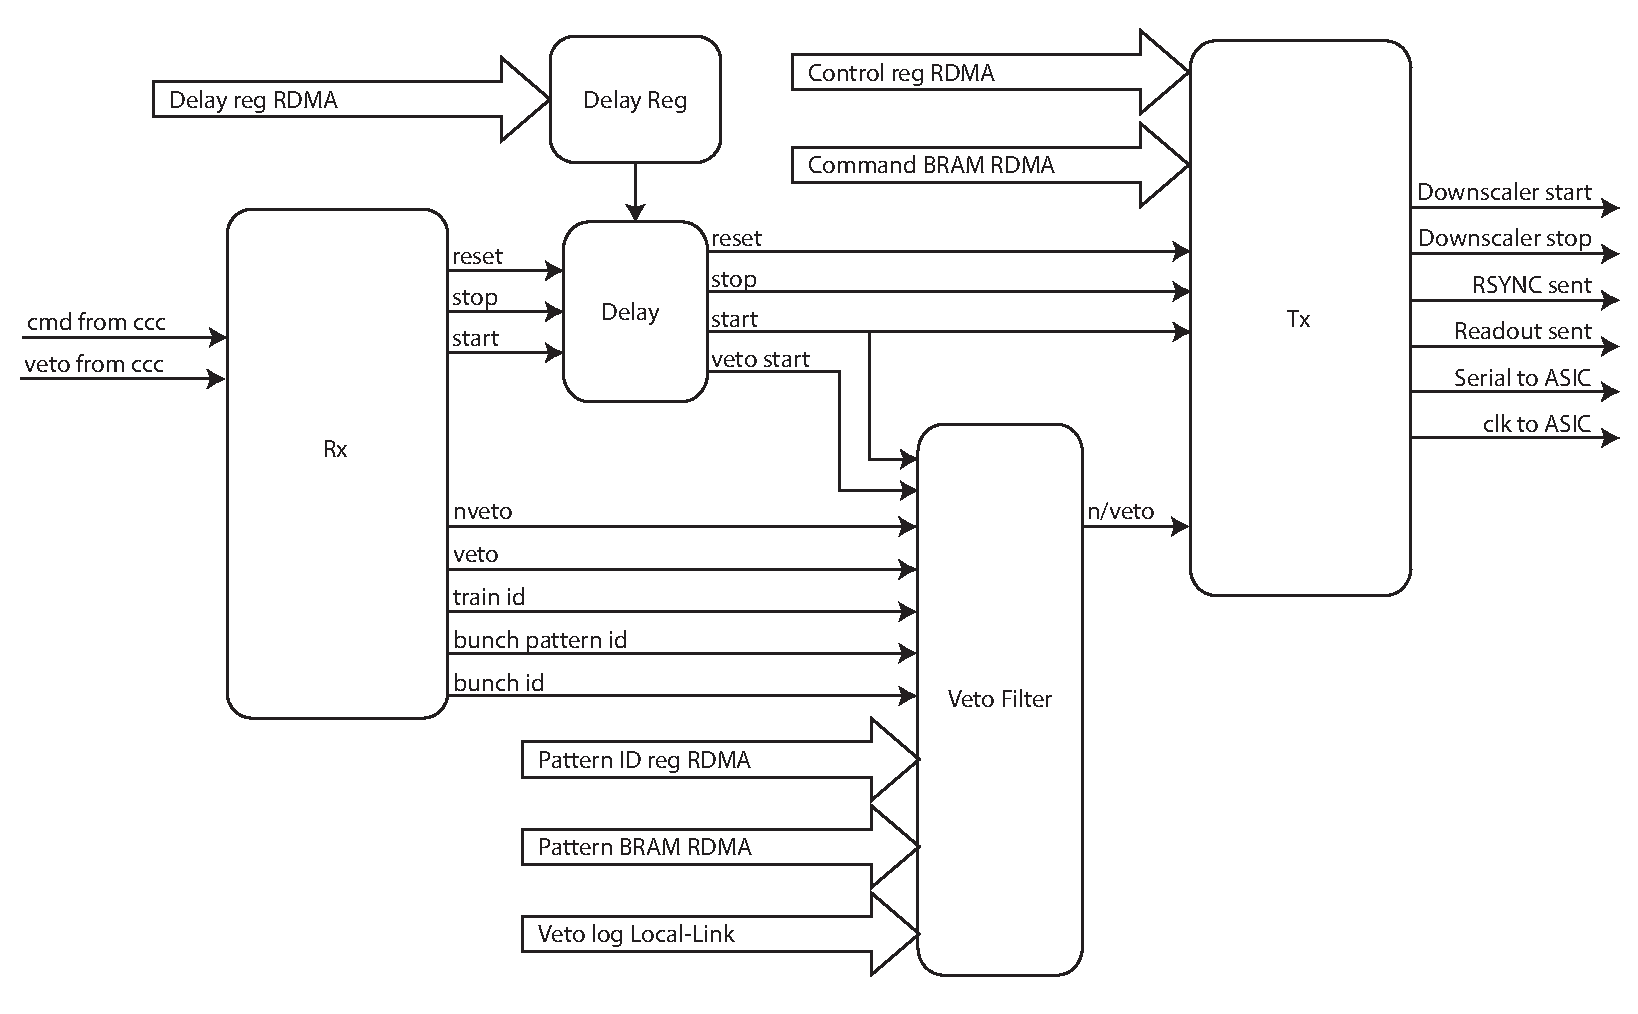
\includegraphics[width=\textwidth]{images/pdfs/ccc_interface_block.pdf}
  \caption{Top level block diagram.}
  \label{fig:ccc_interface_entity}
\end{figure}
    
% subsection top_implementation (end)
% section top_level (end)
%%%%%%%%%%%%%%%%%%%%%%%%%%%%%%%%%%%%%%%%%%%%%%%%%%%
\section{Receiver} % (fold)
\label{sec:receiver}
As stated in the introduction there are five signals that are sent by the CCC, these are transmitted via two ports: the \texttt{cmd\_from\_ccc} and the \texttt{veto\_from\_ccc}. The CCC \texttt{clk} carries the derived fast clock (normally 99~MHz) which is synchronised to the slow machine clock (normally 4.5~MHz) which is distributed by the timing receiver. The full list of commands and payloads can be seen in table~\ref{tab:ccc_commands}. As the receiver block is expected to be static during operation (i.e.\ not need any configuration) only generics are used and there are now externally accessible registers.
\begin{table}[htbp]
  \begin{center}
  \begin{tabular}{c | c | c | c}
    Name     & Value & Payload & Notes \\
    \hline
    START    & 0b1100 & 48b                 & Start of the train \\
    STOP     & 0b1010 & n\textbackslash a   & End of the train \\
    RESET    & 0b1001 & n\textbackslash a   & Reset the FEM and ASIC \\
    \hline
    VETO     & 0b110  & 8b                  & Veto this bunch \\
    NO-VETO  & 0b101  &                     & Record this bunch \\
  \end{tabular}
  \end{center}
  \caption{The full set of commands received from the CCC. The payload for the \texttt{START} is the train ID (32b), the bunch pattern ID (8b) and a check-sum (8b). The (\texttt{NO-})\texttt{VETO} payloads are the same an 8b bunch ID.}
  \label{tab:ccc_commands}
\end{table}

\subsection{Interface} % (fold)
\label{sub:rx_interface}
The top level interface for the receiver entity is shown in table~\ref{tab:rx_interface}. Of the generics only the word definitions should be changed and only then for words of the same length (e.g.\ `110' changed for `101'). The payload values can be made shorted but not longer.
    
The in ports are essentially the same as the CCC specification with the addition of an internal asynchronous \texttt{rst} line which will clear any buffers and return the state-machines to IDLE.
    
The outputs give a single line for each command as well as buses that hold payload values until over written. It's important to note that the command lines go high for only a single clock whilst the payload buffers will retain their value until the next command starts, this means that, for example, the train\_id will remain available until the \texttt{STOP} command begins to be received.
\begin{table}[htbp]
  \begin{center}
    \begin{tabulary}{\textwidth}{l|c|c|L}
      Name          & Direction & Type       & Description \\
      \hline
      START\_WORD            &  &  slv (3:0) & Default serial command: 1100\\
      STOP\_WORD             &  &  slv (3:0) & Default serial command: 1010         \\
      RESET\_WORD            &  &  slv (3:0) & Default serial command: 1001         \\
      VETO\_WORD             &  &  slv (2:0) & Default serial command: 110          \\
      NO\_VETO\_WORD         &  &  slv (2:0) & Default serial command: 101          \\
      BUNCH\_ID\_LENGTH      &  &  integer   & Expected bunch ID length (default:12)\\
      TRAIN\_ID\_LENGTH      &  &  integer   & Expected train ID length (default:32)\\
      CHECKSUM\_LENGTH       &  &  integer   & Expected checksum length (default:8) \\
      BUNCH\_PATTERN\_LENGTH & \multirow{-9}{*}[11.5pt]{Generic} 
                                &  integer   & Expected bunch pattern ID length (default:8) \\
      \hline
      clk          & \multirow{4}{*}{in}  & sl                & CCC clock \\
      rst          &   & sl                & FEE internal reset              \\
      cmd\_i       &   & sl                & Fast command line from CCC      \\
      veto\_i      &   & sl                & Fast veto line from CCC         \\
      \hline
      start\_o     & \multirow{8}{*}{out} & sl                & Start signal to transmitter     \\
      stop\_o      &  & sl                & Stop signal to transmitter      \\
      rst\_o       &  & sl                & Reset signal for transmitter    \\
      veto\_o      &  & sl                & Veto to trigger veto filter     \\
      no\_veto\_o  &  & sl                & No veto to trigger veto filter  \\
      bunch\_p\_o  &  & slv (7:0)  & Bunch pattern ID to veto filter \\
      bunch\_id\_o &  & slv (7:0)  & Bunch ID to veto filter         \\
      train\_o     &  & slv (31:0) & Train ID to veto filter         \\
    \end{tabulary}
  \end{center}
  \caption{Top level interface of the receiver entity.}
  \label{tab:rx_interface}
\end{table}
% subsection interface (end)
\subsection{Implementation} % (fold)
\label{sub:rx_implementation}
The receiver module is split into two state machines, one for each of the two command lines, as seen in figure~\ref{fig:rx_entity}. The entities have similar designs although the command receiver entity is slightly more complex to cope with the non-constant, multi-part payloads. 
\begin{figure}[htbp] 
  \centering
  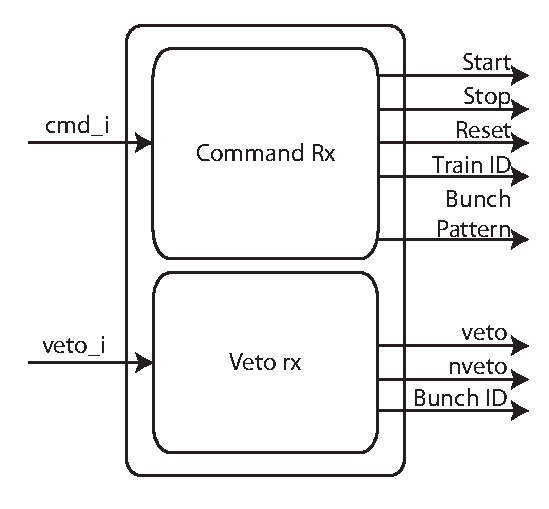
\includegraphics[scale=1]{images/pdfs/rx_block.pdf}
  \caption{Block diagram of the receiver entity.}
  \label{fig:rx_entity}
\end{figure}
  
The designs uses strobes to signal which type of command has been received and buses to hold the ID information. The ID-buses (train, bunch pattern, checksum and bunch) are cleared at the start of the next command, this means that the data is available until it gets replaced.
  
The two entities use simple state-machines designs (figures~\ref{fig:cmd_rx_flow} and \ref{fig:veto_rx_flow}) that can be summarised as: `IDLE \( \rightarrow \) LOG\_COMMAND \( \rightarrow \) STROBE\_COMMAND \( \rightarrow \) [LOG\_PAYLOAD \( \rightarrow \)] IDLE'. For both command and veto lines the state machine is triggered by the line going high. The stream is de-serialised by passing the serial commands to a shift register once a command is matched then the appropriate strobes is set. If the command has an attached payload then that is passed to a shift register until the appropriate number of payload bits have been received when they are written to a bus and the machine returns to `IDLE'.
\begin{figure}[htbp]
  \centering
  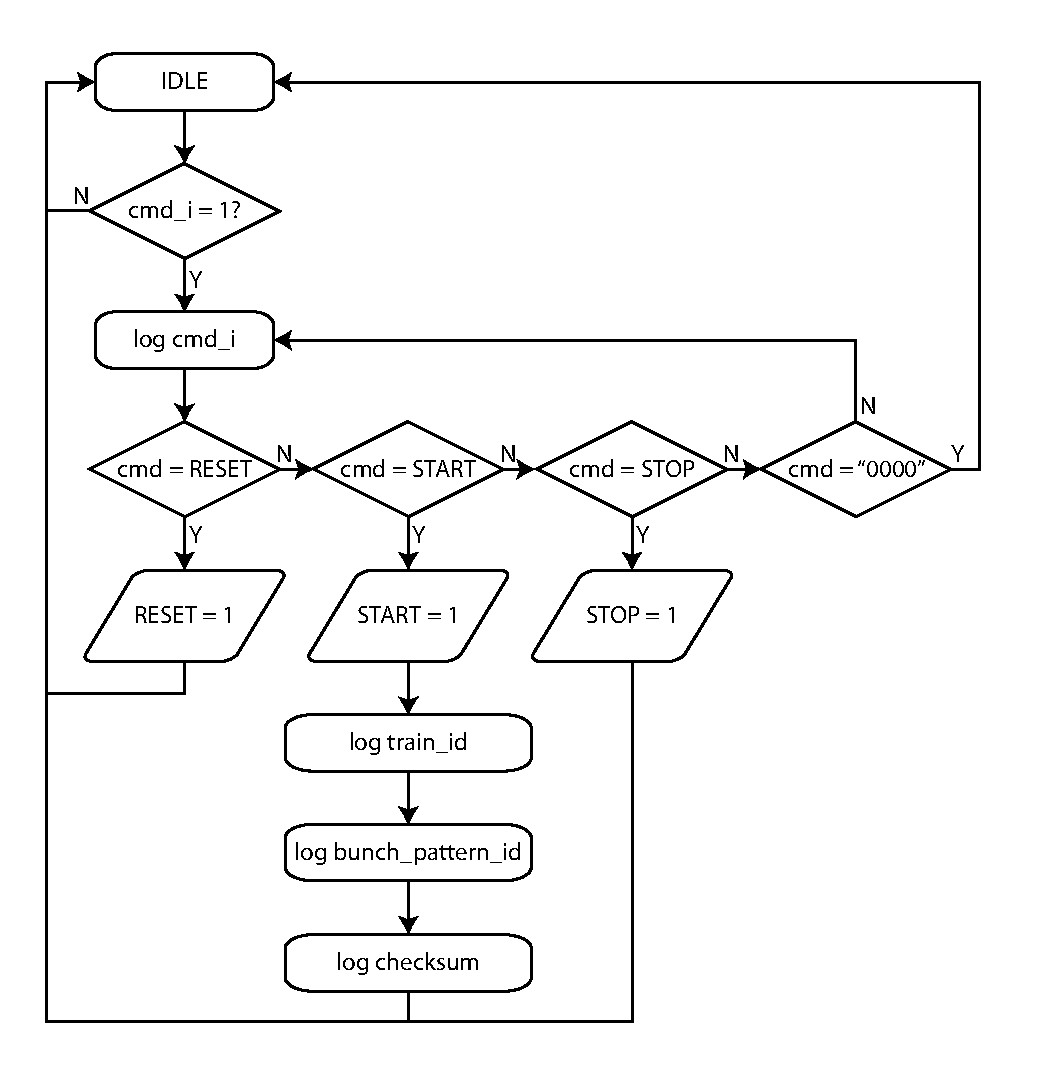
\includegraphics[width=0.7\textwidth]{images/pdfs/cmd_rx_flow.pdf}
  \caption{Flow diagram of the command receiver. The serial signals are read and flags set as required. The `START' payload (i.e. train ID, bunch pattern ID and checksum) are stored and remain available until cmd\_i next goes high (i.e. the start of the next command).}
  \label{fig:cmd_rx_flow}
\end{figure}
\begin{figure}[htbp]
  \centering
  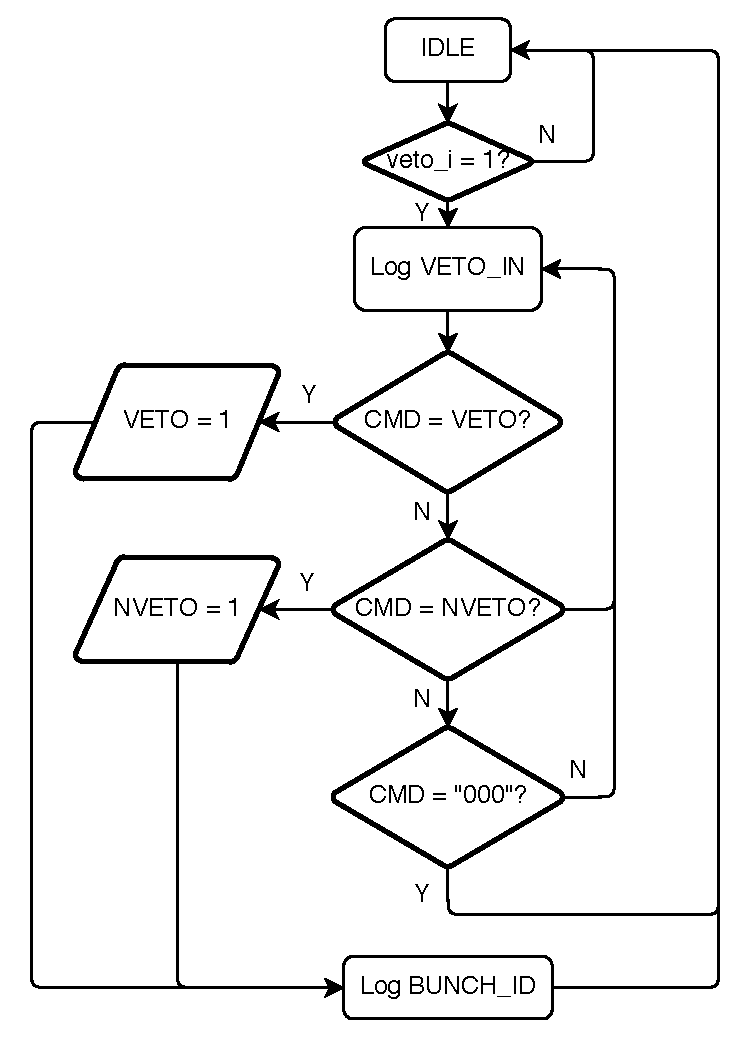
\includegraphics[width=0.5\textwidth]{images/pdfs/veto_rx_flow.pdf}
  \caption{Flow diagram of the veto receiver entity. This de-serialises and splits the veto signals into the command and its payload, the bunch id.}
  \label{fig:veto_rx_flow}
\end{figure}

As every command on the \texttt{veto} port has the same format (<\texttt{COMMAND}~3:0><\texttt{BUNCH~ID}~11:0>) the veto receiver (figure~\ref{fig:veto_rx_flow}) only implements two states: CMD and BUNCH\_ID with the command (either VETO or NO-VETO) being flagged once it's received and the bunch ID being recorded regardless. In the command receiver (figure~\ref{fig:cmd_rx_flow}) there are five states: IDLE, CMD, TRAIN, BUNCH\_PATTERN and CHECKSUM. The TRAIN, BUNCH\_PATTERN and CHECKSUM are used to record the \texttt{START} command's payloads. If the \texttt{STOP} or \texttt{RESET} commands are received the flow returns to IDLE to await the next command. 
% subsection implementation (end)
% section receiver (end)
%%%%%%%%%%%%%%%%%%%%%%%%%%%%%%%%%%%%%%%%%%%%%%%%%%%
\section{Veto Filter} % (fold)
\label{sec:veto_filter}
As discussed in section~\ref{sub:veto_signal} there are two sources of vetoes that needed be combined: the bunch pattern and the online sources. It is assumed that 10 bunch patterns will be sufficient for general operation. The LPD, due to its fixed pipeline size, has a third source of vetos: only 512 bunches can be recorded.\footnote{Unless running with a single gain setting.} A general truth table is given in table~\ref{tab:veto_truth_table}, as can be seen a \texttt{NO-VETO} is only sent if fewer than the maximum \texttt{NO-VETOS}s have been sent and both the pattern and the veto line agree specify that a \texttt{NO-VETO} should be sent.
    
\begin{table}[htbp]
  \begin{center}
    \begin{tabular}{r|r|r||r}
      Line  & Pattern &   Count   & Outcome \\
      \hline
      veto  &   veto  & \(>\) Max & veto    \\
      nveto &   veto  & \(>\) Max & veto    \\
      veto  &  nveto  & \(>\) Max & veto    \\
      nveto &  nveto  & \(>\) Max & veto    \\
      \hline
      veto  &   veto  & \(<\) Max & veto    \\
      nveto &   veto  & \(<\) Max & veto    \\
      veto  &  nveto  & \(<\) Max & veto    \\
      nveto &  nveto  & \(<\) Max & no-veto \\
            
    \end{tabular}
  \end{center}
  \caption{Truth table for veto decisions. Count is the number of `no-veto's already sent, it assumed to be 512 but can be any number less than this.}
  \label{tab:veto_truth_table}
\end{table}

\subsection{Interface} % (fold)
\label{sub:veto_interface}
The interface for the veto filter is given in table~\ref{tab:veto_interface}. There are ten generics to be set that specify the reset values for the pattern ID register (see section~\ref{sub:pattern_id_registers}).
    
The in ports are mainly concerned with signals from the receiver module, these are used to determine when vetoes should be expected as they need to be synchronised with the bunch clock. There are two start signals that are of concern: the \texttt{veto\_start} and \texttt{start\_i}, the former of these indicates when the first veto should be expected whilst the latter indicates that the \texttt{START} command, the train~ID and the bunch~pattern~ID have been received. The train and bunch~pattern~IDs are required before the first veto is received in order to correctly load the veto pattern as well as create the header for the veto logger. The bunch~ID is received but, currently, nothing is done with it. The \texttt{stop\_i} signal is used as an alternative to the maximum number of bunches to stop the veto filter.
    
The out ports are very simple, one is the final veto decision which is sent to the transmitter whilst the other is a count of the number of \texttt{NO-VETO} commands sent to the ASIC. The number of no-vetoes is required for the read-out entity to know how many words to expect once read-out starts.
    
There are 3 data interfaces which are discussed in section~\ref{sub:tx_registers}. Briefly: the two RDMA interfaces allow external access to the pattern BRAM and the pattern ID register whilst the LocalLink interface is used by the read-out entity to access the veto-decision-log which is required for data reconstruction.
    
\begin{table}[htbp]
  \begin{center}
    \begin{tabulary}{\textwidth}{l|c|c|L}
      Name & Direction & Type & Description \\
      \hline 
      WORD\_LENGTH               & & integer                   & Length of ASIC command word (default: 22).           \\
      MAX\_NVETOS                & & integer                   & Number of n\_vetos we can send (default: 512).       \\
      N\_BUNCHES                 & & integer                   & Maximum number of bunches in a train (default: 3072).\\
      % PATTERN\_REG\_(0:9)\_RESET & & slv (31:0) & Reset values for the pattern register (default: see~\ref{sub:veto_registers}). \\
      PATTERN\_REG\_(0:9)\_RESET &  \multirow{-4}{*}[-11.5pt]{generic} 
                                   & slv (31:0) & Reset values for the pattern register (default: see~\ref{sub:veto_registers}). \\
      \hline
      clk                & \multirow{10}{*}[-5.75pt]{in}  
                           & sl                & CCC clock.          \\
      rst                & & sl         & Internal FEE reset.                             \\
      veto\_i            & & sl         &                                                 \\
      nveto\_i           & & sl         &                                                 \\
      start\_i           & & sl         &                                                 \\
      stop\_i            & & sl         &                                                 \\
      veto\_start        & & sl         & Delayed start signal to coincide with vetos.    \\
      bunch\_id          & & slv (11:0) & Not actually used.                              \\
      train\_id          & & slv (31:0) & Added to the local link header.                 \\
      bunch\_pattern\_id & & slv (7:0)  & Used to select the veto pattern.                \\
      \hline   
      veto\_to\_tx       & \multirow{2}{*}[-11.5pt]{out} 
                            & sl                & Combined pattern and veto decision.             \\
      nvetos\_sent       &  & slv (8:0)  & Need to know how much to read from the ASIC.    \\
      \hline
      pattern\_bram\_rdma     & \multirow{3}{*}[-23pt]{interface} 
                                 & RDMA      & Interface to the pattern entity RAM, mask: 0x000003FF \\
      pattern\_id\_reg\_rdma  &  & RDMA      & Interface to the pattern ID/BRAM offset registers, mask: 0x0000000F. \\
      ll                      &  & LocalLink & Interface to the veto log FIFO, uses a 256b data bus. \\
    \end{tabulary}
  \end{center}
  \caption{Interface for the veto filter.}
  \label{tab:veto_interface}
\end{table}
% subsection veto_interface (end)
\subsection{Registers} % (fold)
\label{sub:veto_registers}
In the veto filter there are two memory blocks: the pattern ID registers and pattern BRAM, both accessed via a dedicated RDMA interface and the veto log which is accessed via local link (see appendices~\ref{app:rdma_interface} and~\ref{app:local_link_interface}). 
\subsubsection{Pattern BRAM} % (fold)
\label{sub:pattern_bram}
The pattern BRAM holds the pre-defined veto patterns. These are combined with the fast veto line to decide whether or not to veto a bunch (i.e. a bunch can be vetoed by either the pattern \emph{or} the veto line). Each pattern consists of a bit for each bunch in a train (it is assumed that there will be \( < \)3,072 bunches in each train). If the corresponding bit is `1' then the bunch will be vetoed, otherwise it is dependant on the veto line.
  
It is assumed that no more than ten patterns will be needed in normal operation so the BRAM is configured to hold 1,024\( \times  \)32b words. This means that for a 3,072 bunch train 96 words need to be defined for each pattern. The pattern is assumed to be spread across monotonically increasing addresses (e.g. address 0x0 to 0x60), the veto bits are applied 0 to 31. 
% subsubsection pattern_bram (end)
\subsubsection{Pattern ID registers} % (fold)
\label{sub:pattern_id_registers}
The pattern ID registers map IDs to their appropriate offset within the BRAM. The specifications do not define the number of patterns needed during normal operation but it is assumed to be (\( < \)10); there are therefore 10 registers given to providing the required mapping one register per bunch pattern used. The value of each register must be of the format:
\begin{align} \label{fmt:pattern_id}
  <\text{PATTERN\_ID } 31:24>\ldots<\text{BRAM offset } 9:0> 
\end{align}
Default values for the register are given in table~\ref{tab:default_pattern_id_reg}, the reset values are set via generics at the top level and the current value can be changed via RDMA. The defaults assume that the patterns are all unique with no overlap, as such each delimitates 96\( \times \)32b words i.e. 3,072 bunches. If there is an intersection between the end of one pattern and the start of another then setting the offset to the beginning of the common section will work as expected.
\begin{table}[htbp]
  \begin{center}
    \begin{tabular}{c|c|c|c}
      Register & Value      & Pattern ID & Offset \\
      \hline
      0x1      & 0x01000000 & 0x1        & 0x000  \\ 
      0x2      & 0x02000060 & 0x2        & 0x060  \\  
      0x3      & 0x030000C0 & 0x3        & 0x0C0  \\ 
      0x4      & 0x04000120 & 0x4        & 0x120  \\ 
      0x5      & 0x05000180 & 0x5        & 0x180  \\ 
      0x6      & 0x060001E0 & 0x6        & 0x1E0  \\ 
      0x7      & 0x07000240 & 0x7        & 0x240  \\ 
      0x8      & 0x080002A0 & 0x8        & 0x2A0  \\ 
      0x9      & 0x09000300 & 0x9        & 0x300  \\ 
      0xA      & 0x0A000360 & 0xA        & 0x360  \\ 
    \end{tabular}
  \end{center}
  \caption{Default reset values for pattern ID registers.}
  \label{tab:default_pattern_id_reg}
\end{table}
% subsubsection pattern_id_registers (end)
\subsubsection{Veto log} % (fold)
\label{sub:veto_locallink}
The veto log is a 13\( \times \)256b FIFO which logs the veto decision for each bunch. This information is formed into a LocalLink frame which uses 256b data words. The 256b header is defined as:
\begin{align}\label{fmt:ll_header}
  <\text{Train ID } 255:224><\text{Bunch Pattern ID } 223:216>\ldots<\text{Number of no-vetos sent } 191:182> \ldots
\end{align}
where `\( \dots \)' represent padding (1's). The rest of the frame consists of the veto log which consists of a bit per bunch indicating either a veto (`1') or a no-veto (`0'). The entities are ordered MSB first, e.g.\ bit 255 of frame 0 indicates the first veto decision whilst bit 0 of frame 12 indicates the last decision. 
% subsubsection veto_locallink (end)
% subsection veto_registers (end)
\subsection{Implementation} % (fold)
\label{sub:veto_implementation}
The veto filter is split into two distinct processes: filtering and logging. Filtering is a requirement of the specification. The logging is required because the ASIC records no identifying information about each bunch and due to the ASIC's write pointer wrapping through memory, images are not guaranteed to be read out in chronological order, a block diagram of this solution is shown in figure~\ref{fig:veto_filter_entity}.
    
\begin{figure}[htbp]
  \centering
  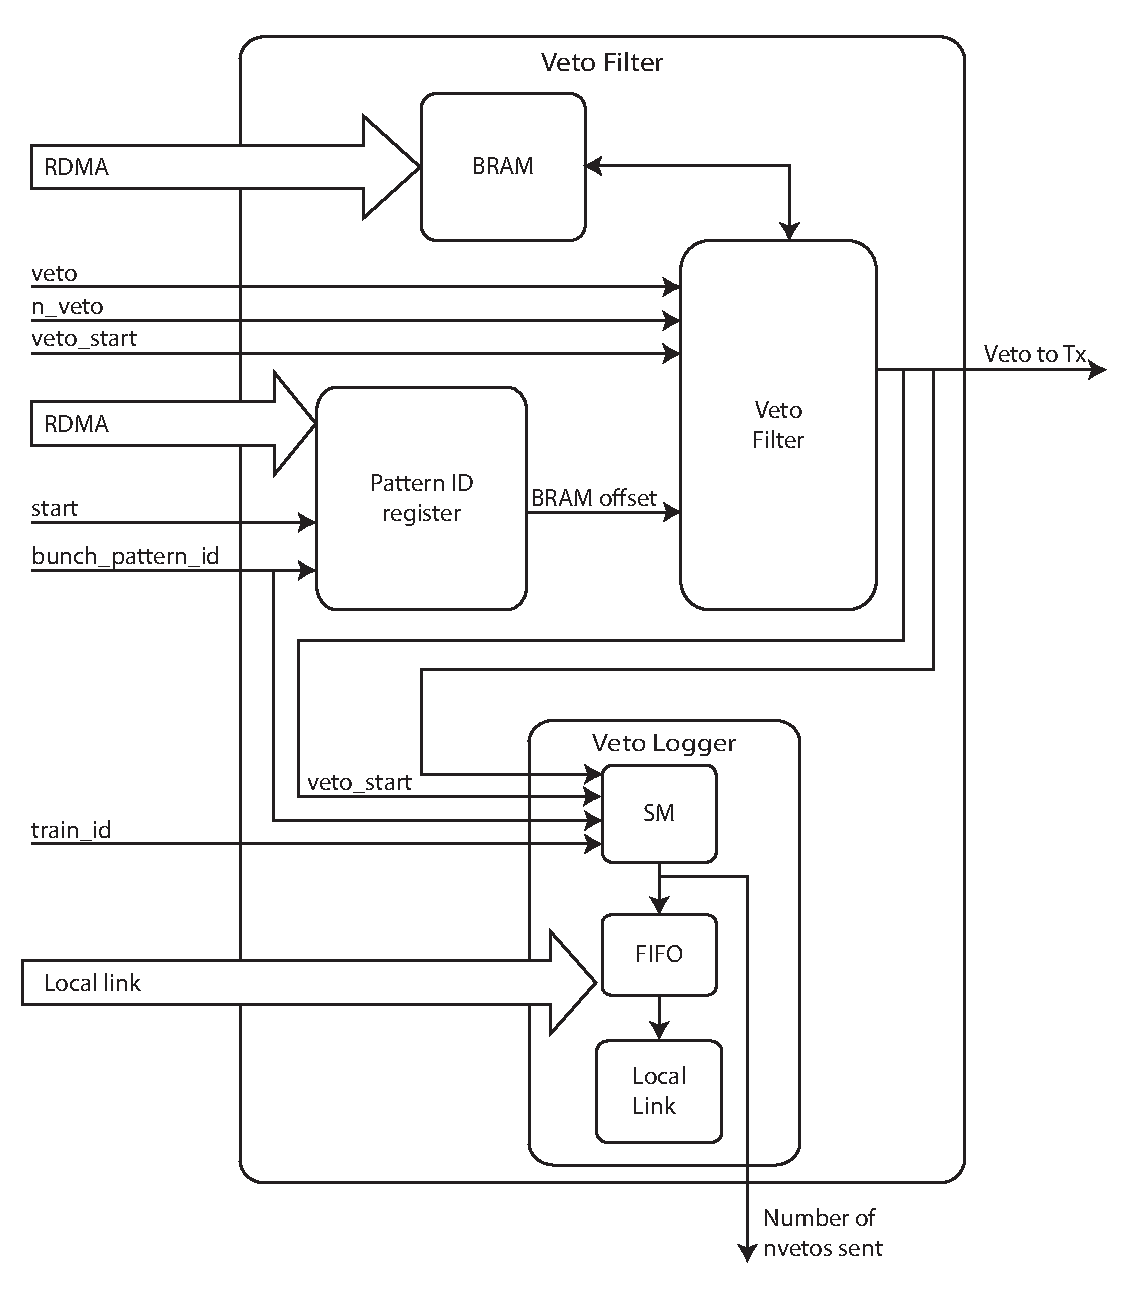
\includegraphics[width=0.7\textwidth]{images/pdfs/veto_filter_block.pdf}
  \caption{Block diagram of the veto filter.}
  \label{fig:veto_filter_entity}
\end{figure}
    
The  1,024\( \times \)32b BRAM is used to store the veto patterns to be combined with the veto signal in order to form the veto decisions. To construct the veto decision and control access into the BRAM a state machine is implementing figure~\ref{fig:veto_filter_flow} was used. The veto decisions are made at the beginning of each word to reduce latency whilst BRAM and state changes are made at the end. The final entity, the pattern ID register, exists to specify the mapping from bunch pattern ID to BRAM offsets.
    
\begin{figure}[htbp]
  \centering
  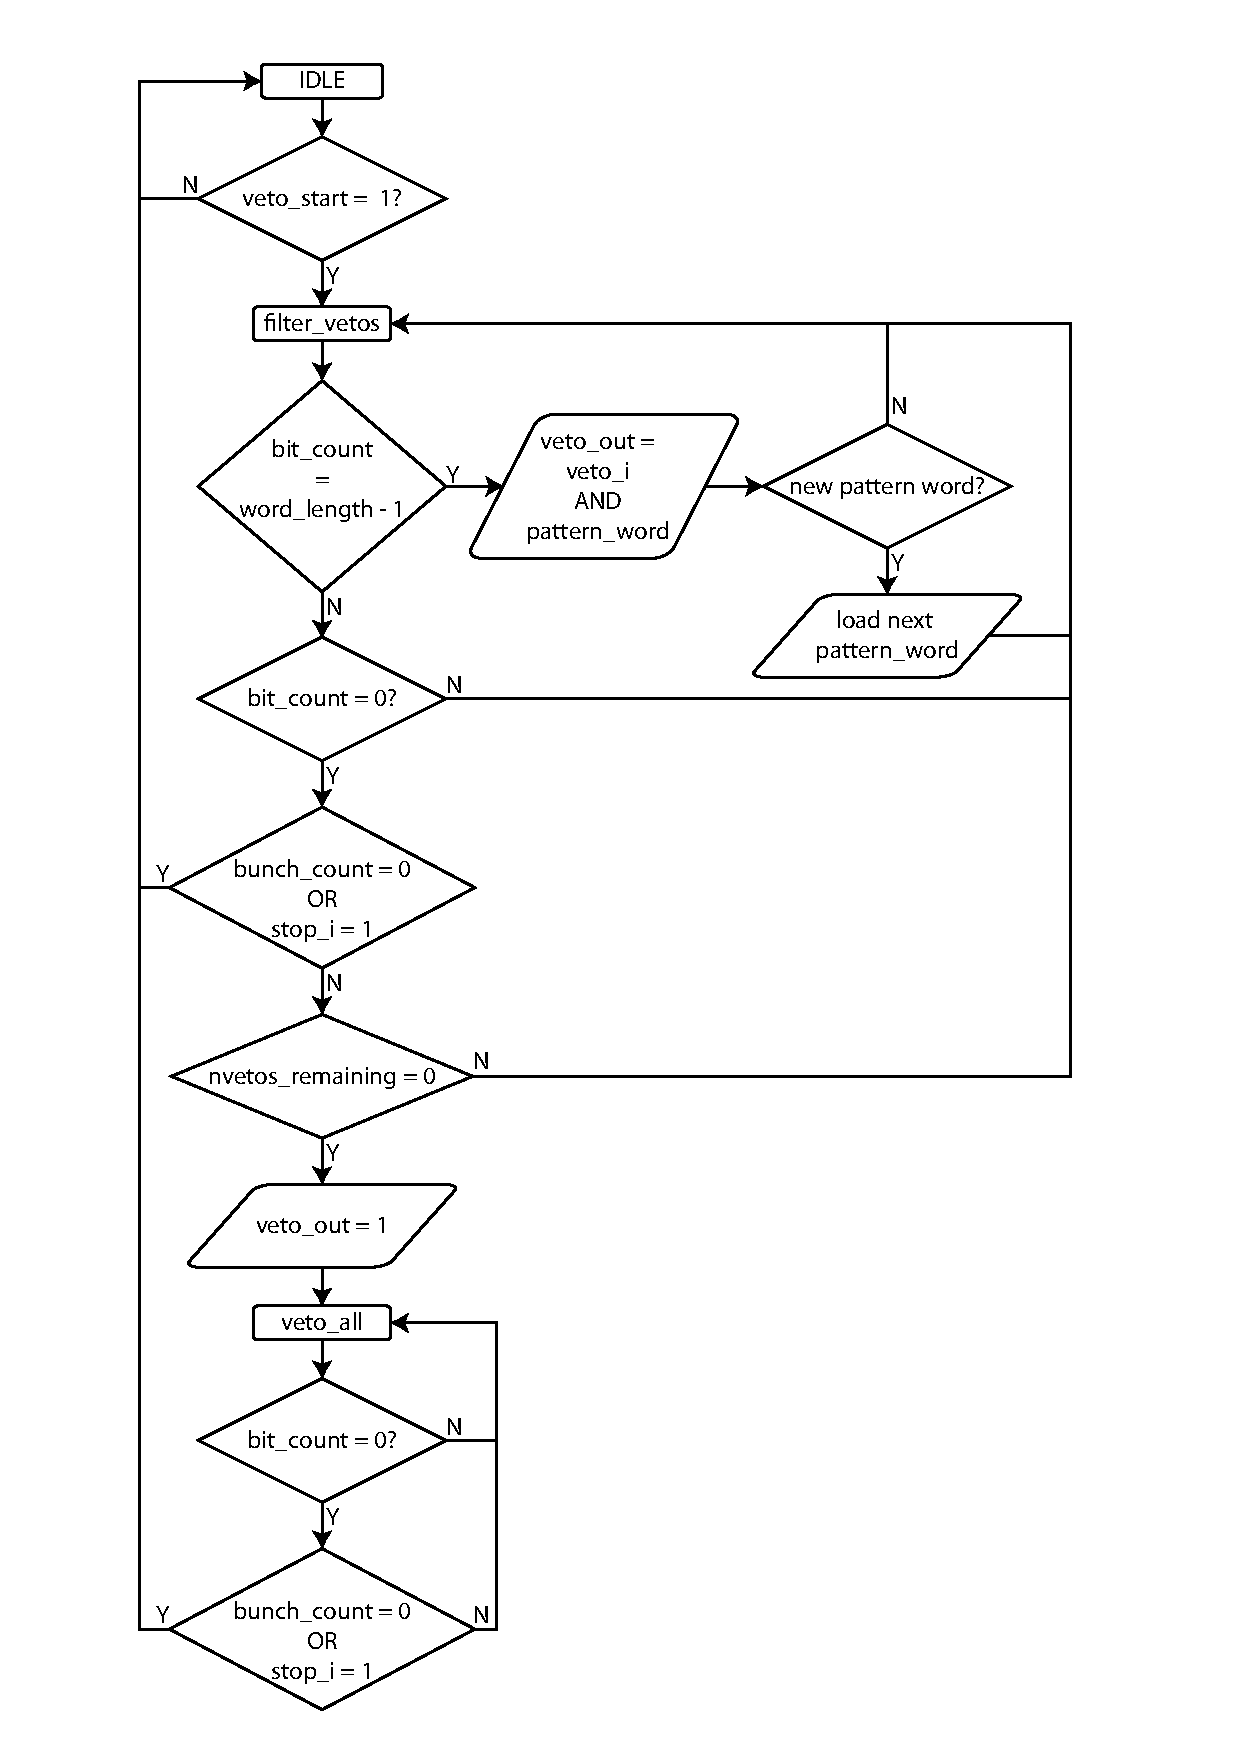
\includegraphics[width=0.8\textwidth]{images/pdfs/veto_filter_flow.pdf}
  \caption{Flow diagram of the veto filter.}
  \label{fig:veto_filter_flow}
\end{figure}
    
The logging is performed using a simple state machine to feed in words to a 32b in, 256b out first in, first out BRAM (FIFO), this state machine (figure~\ref{fig:veto_logger_flow}) also constructs the LocalLink frame header (the train ID, the bunch ID then `0' padding). The header requires 8 clocks between \texttt{start\_i} being asserted and \texttt{veto\_start}, to be properly formed. The FIFO is a simple First Word Fall Through (FWFT) entity with the optional \texttt{empty} and \texttt{almost\_empty} signals enabled. The read out of the FIFO is performed via a 256b-word LocalLink interface. Once either \texttt{stop\_i} is asserted or \texttt{N\_BUNCHES} have been counted any remaining bits of the 256b word are filled with `1's and the LocalLink's \texttt{src\_rdy} is asserted. 
    
The LocalLink interface is implemented by wrapping the FIFO's 256b \texttt{data\_out} port in some simple logic to make it conform to the local link standard. This mainly involves using \texttt{empty} to monitor the state of the FIFO, \texttt{almost\_empty} as \texttt{eof} and an internal flag from the logging state-machine for the \texttt{sof}. The \texttt{sop} (start-of-payload) signal is not used to differentiate the header from the payload as the entire frame will ultimately form part of the meta-data in the header of the read-out.
    
\begin{figure}[htbp]
  \centering
  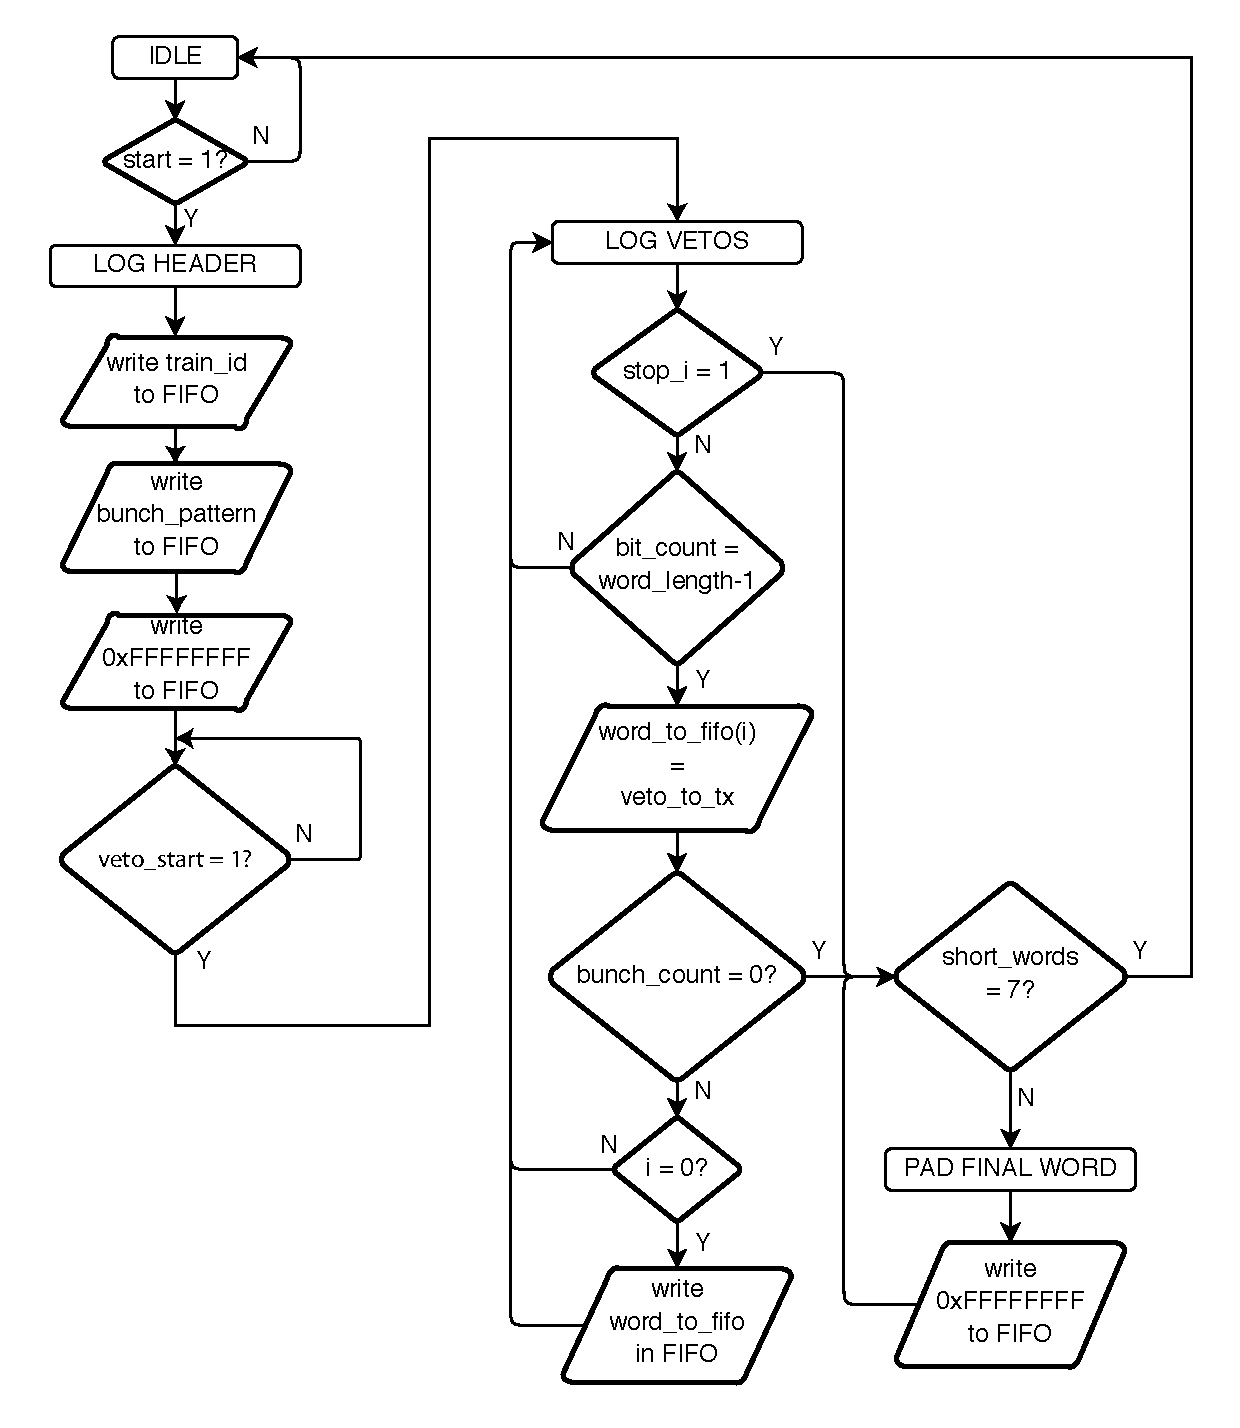
\includegraphics[width=0.8\textwidth]{images/pdfs/veto_logger_flow.pdf}
  \caption{Flow diagram for the veto decision logger.}
  \label{fig:veto_logger_flow}
\end{figure}

% subsection veto_implementation (end)
% section veto_filter (end)
%%%%%%%%%%%%%%%%%%%%%%%%%%%%%%%%%%%%%%%%%%%%%%%%%%%
\section{Transmitter} % (fold)
\label{sec:transmitter}
The transmitter entity's main task is to act as the interpreter for the signals received from the CCC, translating them into command sequences that the ASIC can understand and act upon. As has been discussed above there are four signals that need to be translated for the ASIC: \texttt{START}, \texttt{STOP}, \texttt{RESET} and (\texttt{NO-})\texttt{VETO}. The first three command signals all require an arbitrary number of words be sent to the ASIC whilst the veto signals are responded to by one of two words.
    
The transmitter can run in one of two mode: `dynamic veto mode' and `reset mode'. Dynamic veto mode is intended to be the normal mode of operation for XFEL whilst reset mode is intended for static runs with simple veto patterns (e.g.\ for testing). A comparison of the two can be seen in table~\ref{tab:dynamic_vs_reset_mode}. Reset mode is enabled by strobing bit 0 of the main control register (see section~\ref{sub:ctrl_reg} for details). The transmitter also has an optional minor mode called `down-scaler mode' this is primarily for v~1.0 of the ASIC that requires a slower clock during readout. When enabled it uses a multiplier (set by generic) to slow slow the clock, after a set number of cycles normal speed is resumed. 
    
\begin{table}[htbp]
  \begin{center}
    \begin{tabular}{r | X{2.5cm} | X{2.5cm} }
      & \multicolumn{2}{c}{Mode} \\
      & Dynamic-veto & Reset \\
      \hline
      Standalone operation   & \xmark & \cmark \\
      Dynamic veto decisions & \cmark & \xmark \\
      \multirow{4}{*}{Signal response}
      & START  & \multirow{4}{*}{Register flag} \\
      & STOP   & \\
      & RESET  & \\
      & N/VETO & 
    \end{tabular}
  \end{center}
  \caption{Comparison of dynamic veto and reset modes}
  \label{tab:dynamic_vs_reset_mode}
\end{table}

\subsection{Controlling the ASIC} % (fold)
\label{sec:controlling_the_asic}

The LPD ASIC manual~\cite{lpd_manual} specifies the command sequences required for each stage of operation of the ASIC. For the veto commands a simple selection between \texttt{NOP} (veto) and \texttt{TRIGGER\_FLAG\_SET} (no-veto) is required, the other commands have more complex sequence sets that can change based on operation a brief summary will be given here full details can be found in the LPD ASIC manual~\cite{lpd_manual}. 

The standard response to the START command is to set the ASIC in a state ready to write to its memory, this means reseting the write and trigger points and clearing the skip register. Once these commands have been carried out the ASIC will start incrementing the write pointer through the memory locations after additionally starting the trigger pointer the ASIC is ready to write the contents of the pixels when a \texttt{TRIGGER\_FLAG\_SET} (i.e.\ NO-VETO) is received. 

The command sequence for the STOP command is more complex and split over two stages: the pre and post readout sections. To start readout the ASIC is set in a stable mode thus:
\begin{enumerate}
  \item The ASIC is put in power saving mode.
  \item Read out of the data begins.
  \item Disable on-chip resets.
  \item Manually reset the gain, pre-amp, write and trigger pointers.
\end{enumerate}
The data read back consists of one 36b word for each no-veto sent, once all of these have been sent the ASIC is returned to ready mode for the next train:
\begin{enumerate}
  \item Power up the ASIC, i.e.\ return bias currents to full
  \item Re-synchronise the ASIC to the bunch (\( \sim \)4.5~MHz) clock.
  \item Re-enable on chip resets.
  \item Stop read out.
\end{enumerate}
\textbf{NOTE:} the above constitute a basic over view of the STOP process, there are some important considerations with regards to synchronisation of these commands that are beyond the scope of this and covered in full in the LPD ASIC manual~\cite{lpd_manual}.

The ASIC command words have the format:
\begin{align}\label{fmt:asic_format}
  <\text{SYNC }19><\text{X }18<\text{CMD } 17:10><\text{PADDING\_ZEROS } 9:0>
\end{align}
if a word length greater than 20b is being used (e.g.\ 22b, the current default) then the zero-padding is extended as required. The `SYNC' bit is a `1' and `X', by convention, a `0' these are automatically prepended by the state machine. The only exception to this is the 20b command \texttt{SYNC\_RESET} (currently set to be 0x5A5A5) which overrides the above format.

% section controlling_the_asic (end)
\subsection{Interface} % (fold)
\label{sub:tx_interface}
The transmitter has three `sets' of generics: the control register reset values, the flag words (ending in \texttt{\_SIG}) and the down-scaler factor. The register resets set the default value to be written to the assorted registers if \texttt{rst} is asserted. The flag words specify certain command words that the transmitter should scan for in order to flag them for use elsewhere. The \texttt{SYNC\_RESET} flag is intended for use with any entities (e.g.\ the slow command line) that have to be synchronised to the ASIC's bunch clock. The \texttt{READOUT} is intended for use by the read-out entity in order to prepare for read-out. The \texttt{DOWNSCALER\_SIG} is used to begin either the internal (if it's enabled) or an external down-scaler clock. The \texttt{DOWNSCALER\_STOP\_SIG} is only for use by an external source (the internal version counts clocks). The \texttt{DOWNSCALER\_FACTOR} specifies the factor to use for the internal down-scaler e.g.\ a factor of 100 means a scale of 100 fast clock cycles to each slow clock.
    
The in ports to the transmitter are all flags from the receiver; with the standard exception of \texttt{rst} which is the FEM internal signal (cf.\ \texttt{reset} which is the flag from the receiver).
    
The out ports fall into 3 categories: signals to the ASIC (\texttt{ASIC\_in} and \texttt{clk\_in}), flags (marked \texttt{\_sent}) and \texttt{start\_nwords\_o}. The ASIC commands are defined in the specification. The flags have been discussed above with regards to their generic-defined trigger words. The final out port is a wrapper to the value of the \texttt{start\_nwords} register (see section~\ref{sub:tx_registers}) which is used in setting the delay for \texttt{veto\_start}.
    
The two RDMA interfaces are used for access to the command sequence BRAM and the control registers (sections~\ref{sub:tx_bram} and \ref{sub:tx_registers} respectively).
    
\begin{table}[htbp]
  \begin{center}
    \begin{tabulary}{\textwidth}{l | c | c | L}
      Name & Direction & Type & Description \\
      \hline
      REG\_RESET\_(9:0)     & & slv (31:0) &  Register resets (0-9), see section~\ref{sub:tx_registers}. \\
      SYNC\_RESET\_SIG      & & slv (31:0) & Flag that the \texttt{SYNC\_RESET} command has been sent.                 \\
      READOUT\_SIG          & & slv (31:0) & Flag that the \texttt{READOUT} command has been sent.               \\
      DOWNSCALE\_SIG        & & slv (31:0) & Flag to start the down-scaler (either internal or external).\\
      DOWNSCALER\_STOP\_SIG & & slv (31:0) & Flag to stop the down-scaler.                               \\
      DOWNSCALE\_FACTOR     & \multirow{-6}{*}[11.5pt]{Generic} % Avoids extra newline at top
      % DOWNSCALE\_FACTOR     & \multirow{-16}{*}[11.5pt]{Generic} % Avoids extra newline at top
                              & integer    & Factor for the internal down-scaler, default: 100.          \\
      \hline
      clk   & \multirow{6}{*}{in} 
               & sl & The CCC clock.          \\
      rst   &  & sl & FEE reset.              \\
      start &  & sl & From the receiver entity.\\
      stop  &  & sl & \dittostraight          \\
      reset &  & sl & \dittostraight          \\
      veto  &  & sl & From the veto filter.   \\
      \hline
      % asic\_in                & \multirow{7}{*}[-28.75pt]{out}
      asic\_in                & \multirow{7}{*}{out}
                                 & sl                & Fast serial commands to the ASIC.  \\
      clk\_in                 &  & sl                & Clock to the ASIC.  \\
      readout\_sent           &  & sl                & Readout flag (for ASIC receiver entity).  \\
      rsync\_sent             &  & sl                & \texttt{SYNC\_RESET} flag (for slow control entity).  \\
      downscaler\_start\_sent &  & sl                & Downscaler start flag.  \\
      downscaler\_stop\_sent  &  & sl                & Downscaler stop flag.  \\
      start\_nwords\_o        &  & slv (31:0) & Number of words used for `START' to set veto\_start delay.\\
      \hline
      bram\_rdma & \multirow{2}{*}[-17.25pt]{Interface} 
      & RDMA & Interface to the ASIC command word BRAM. Mask: 0x000003FF. \\
      ctrl\_rdma & & RDMA & Interface to the control register. Mask: 0x0000000F. \\
    \end{tabulary}
  \end{center}
  \caption{Interface for the transmitter.}
  \label{tab:tx_interface}
\end{table}
  
% subsection tx_interface (end)
\subsection{Registers} % (fold)
\label{sub:tx_registers}
There are two externally accessible sets of registers in the transmitter entity, a control register and the command BRAM both are accessed via RDMA (see appendix~\ref{app:rdma_interface}). The control registers direct the flow of the state machine whilst the BRAM stores the instruction sets to be sent to the ASIC. There are 3 commands that the BRAM has instruction sets for: \texttt{START}, \texttt{STOP} and \texttt{RESET}. Obviously these are normally received via the receiver module but the \texttt{RESET} command can also be sent using a toggle in the control register.
\subsubsection{Control register} % (fold)
\label{sub:ctrl_reg}
The control register specifies 10 registers:
\begin{description}
  \item[1] The general state-machine control register that toggles various modes (i.e. whether to use the down-scaler module and manual \texttt{RESET}) as well as how many bits to send downscaled if that mode is enabled.
  \item[2-7] three pairs of registers that store the number of words (shortened to `nw') and offsets for the 3 different instruction sets (i.e. one \emph{-nw} and one \emph{-offset} for each of \texttt{START}, \texttt{STOP} and \texttt{RESET}).
  \item[8] The word to be sent in case of a veto.
  \item[9] The word to be sent in case of a no-veto.
  \item[10] The status register, indicates what state the state-machine is in.
\end{description}
default values and addresses are given in table~\ref{tab:ctrl_reg_default}.
    
The state-machine control register takes values of the following format:
\begin{align} \label{fmt:control_reg}
  <\text{DOWNSCALER\_ENABLE } 32>\ldots<\text{DOWNSCALER\_BITS } 20:5>\ldots<\text{RESET\_MODE\_EN } 0>
\end{align}
\texttt{reset\_mode\_en} is a flag to manually start the state-machine in reset mode i.e. \texttt{reset\_nwords} worth of commands from \texttt{reset\_offset} in the BRAM will be sent. This mode can be used instead of dynamically determining the veto to be sent in a `fire and forget' manner.

\textbf{DOWNSCALER\_ENABLE} indicates that the internal down-scaler should be used to send the next \textbf{DOWNSCALER\_BITS}, this means that the maximum number of bits that can be sent at the down-scaled rate is \(2^{16} - 1\), i.e. 65,536 or 2,978\(\times\)22b words. Obviously if down-scaling is being handled by an external clock this restriction doesn't apply.

The BRAM offsets and command sequence lengths (\emph{-offset} and \emph{-nw} registers respectively) have maximum values determined by the size of the BRAM i.e.\ 1,024. These values are set using the LSB of the word i.e.\ 9 downto 0. Obviously setting an \emph{-offset} to 1,024 will result in only 1 word and unless the corresponding \emph{-nw} is set to 1 this will result in an address overflow and undefined behaviour. By the same token setting an \emph{-nw} register to 1,024 is allowed but will mean that any other commands to be sent must be either specified as subsets of this command sequence or not used.\footnote{This could be useful if using the reset-mode or in dynamic mode if \texttt{RESET} is not expected to be used.}
    
The veto/no-veto registers specify the appropriate word to send when in dynamic-veto mode, the defaults are \texttt{NOP} and \texttt{TRIGGER\_FLAG\_SET} respectively. When run in this way the state-machine progresses START\(\rightarrow\)vetoes\(\rightarrow\)STOP with vetoes being determined by the veto filter.
      
The status register is a read only register that logs which state the state-machine is in and has the following format:
\begin{align} \label{fmt:status_reg}
  <\text{state\_machine\_enabled } 31>\ldots<\text{RESET } 3> <\text{STOP } 2> <\text{DYNAMIC\_VETO } 1> <\text{START } 0>
\end{align}
	  
\begin{table}[htbp]
  \begin{center}
    \begin{tabular}{c|c | c |c}
      Address & Description             & Reset generic      & Default value  \\
      \hline                    
      0x1     & SM-Control              & CTRL\_REG\_RESET   & 0x00000000     \\ 
      0x2     & Start: offset           & START\_OFF\_RESET  & 0x00000000     \\  
      0x3     & Start: number of words  & START\_NW\_RESET   & 0x00000006     \\ 
      0x4     & Stop: offset            & STOP\_OFF\_RESET   & 0x00000006     \\ 
      0x5     & Stop: number of words   & STOP\_NW\_RESET    & 0x00000007     \\ 
      0x6     & Reset: offset           & RESET\_OFF\_RESET  & 0x0000000D     \\ 
      0x7     & Reset: number of words  & RESET\_NW\_RESET   & 0x0000000F     \\ 
      0x8     & Veto word               & VETO\_WORD\_RESET  & 0x00210000     \\ 
      0x9     & No-veto word            & NVETO\_WORD\_RESET & 0x00200000     \\ 
      0xA     & Status                  & n/a                & 0x00000000     \\ 
    \end{tabular}
  \end{center}
  \caption{Control register layout. With the exception of the status register the reset values of each register can be changed by setting the appropriate reset-generic, these values only take affect when the \texttt{rst} line is asserted \emph{not} when the \texttt{RESET} signal is received.}
  \label{tab:ctrl_reg_default}
\end{table}

% subsubsection control_regsiter (end)
\subsubsection{Instruction set BRAM} % (fold)
\label{sub:tx_bram}
The BRAM used to store the instruction sets is 1,024\(\times\)32b words. Words not defined by the ASIC are ignored so internal flag triggers (e.g. for \texttt{DOWNSCALER\_START}) need not be defined ASIC commands.

The BRAM expects words to have the format:
\begin{align}\label{fmt:tx_bram}
  <\text{N\_NOPS } 31:\text{WORD\_LENGTH }><\text{COMMAND } (\text{WORD\_LENGTH} - 1):0>
\end{align}
The COMMAND is expected to be correctly padded e.g.\ if 22b words are being used for a normal command the last 12b should be `0'. The SYNC bit doesn't need to be set. N\_NOPS indicates how many \texttt{NOP} commands should follow the COMMAND, a NOP is pre-defined to be a SYNC-bit followed by the appropriate number of 0's. It is important to note that NOPs contribute to the number of words sent for any state and a \texttt{NOP} sent as a member of N\_NOPS must not be the final command.

\textbf{Example:} if, for the \texttt{START}-sequence and using 22b words, \texttt{POWER\_UP} (0x02\footnote{see table~\ref{tab:asic_command_words}}) followed by 4 NOPS is to be sent then the first two locations in BRAM could be set to `0x00C08000' and `0x00000000'. 0x00C specifies 3 NOPS (\(\text{0xC}<<2 = 0x3\)\footnote{Where `\(<<\)' is a left-shift, the \( <<2 \) is account for the 2~MSB of the command.}) and 0x08000 is the command (\(\text(0x02) << 22 \)) with the appropriate padding. The final entry of 0x00000000 is the 4\(^{\text{th}}\) NOP; its SYNC bit will be automatically set.
% subsubsection tx_bram (end)
% subsection tx_registers (end)
\subsection{Implementation} % (fold)
\label{sub:tx_implementation}

In order to implement the state machine two concurrent machines are used: the shift-block serialises and inspects command sequences; and the state-machine that determines when to change state and which command sequences to use. Previously, these responsibilities were split across multiple entities but to simplify state sharing and meet the latency requirements they were merged into a single entity. Figure~\ref{fig:tx_entity} shows a entity diagram of the transmitter, both the shift-block and state-machine are within the state-machine entity.
    
\begin{figure}[htbp]
  \centering
  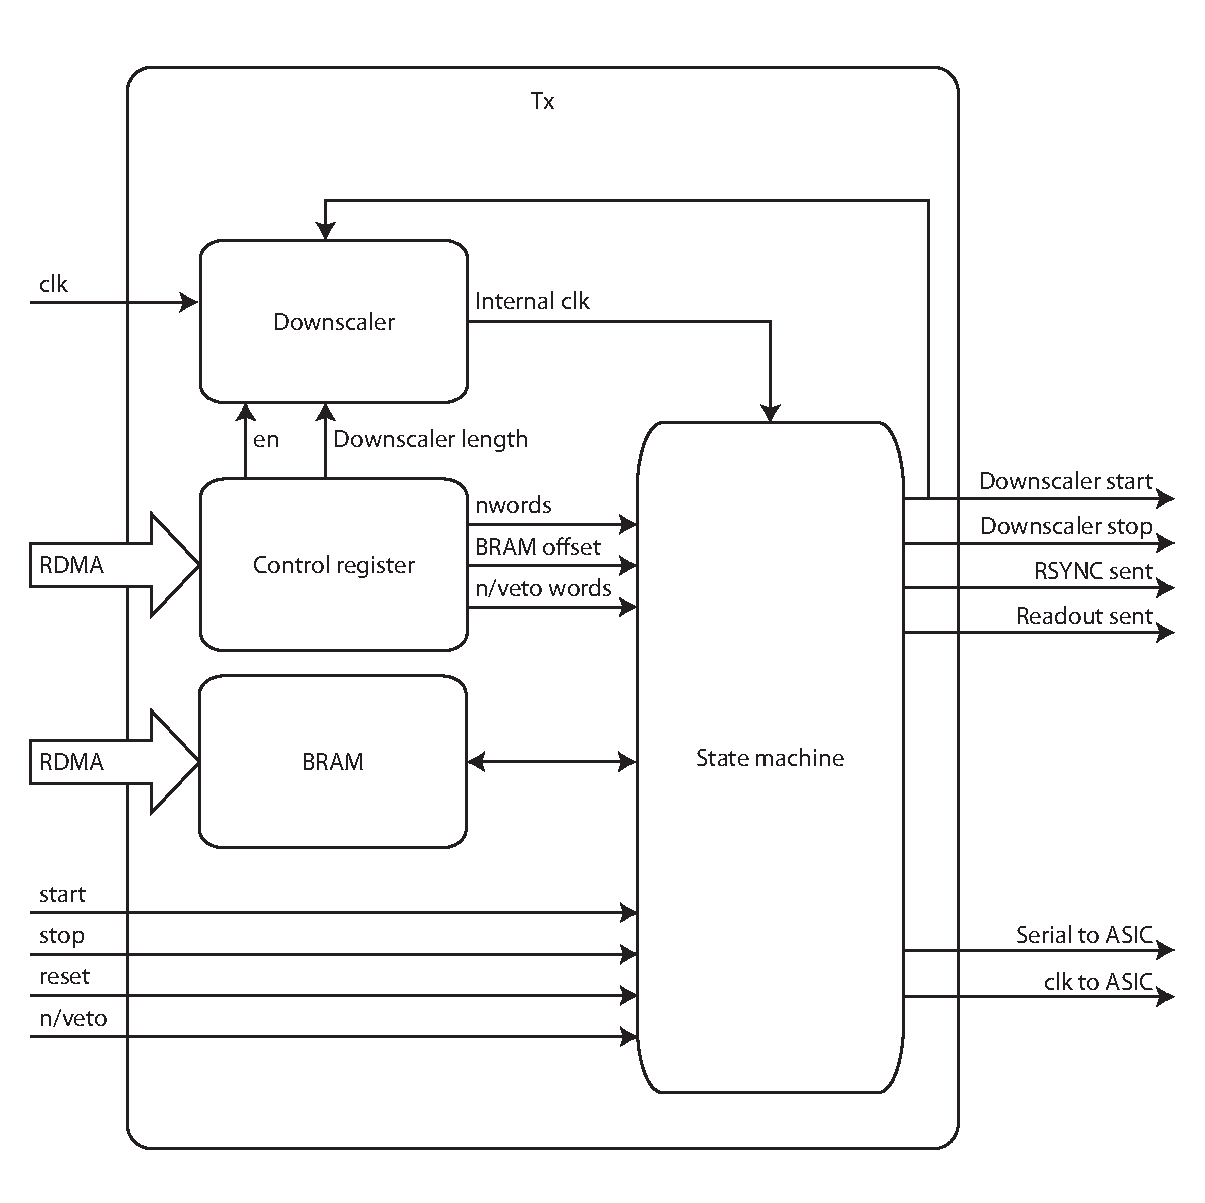
\includegraphics[width=0.8\textwidth]{images/pdfs/tx_block.pdf}
  \caption{Block diagram of the transmitter.}
  \label{fig:tx_entity}
\end{figure}
        
The shift-entity primarily acts as a smart shift register to serialise the command words being sent to the ASIC. It has two secondary functions that require inspection of the commands being serialised: flagging and setting sync-bits. Some of the other components of the FEM require knowledge of when certain command words are sent for their own functionality (e.g. the slow command needs to know when \texttt{SYNC\_RESET} is sent). To do this when a word is loaded from the BRAM (and only from the BRAM) it is compared to the 4 pre-set words given in table~\ref{tab:shift_entity_flags}, if it matches one then the appropriate flag is set. These words are tested sequentially, in the order given in the table, so if a word matches multiple triggers only the flag corresponding to the first match will be set. The flag words are set via generics and are not expected to change, flags do not have to be valid ASIC words although the ASIC's response to unknown commands is undefined and should be confirmed prior to use. At the same time as checking for flags the first two bits of each word are set appropriately: for \texttt{SYNC\_RESET} they are set to 0b01 and all other words 0b10 as specified in \cite{lpd_manual}. These sync-bits are not included in tests for flags. The shift-entity's functionality for the different states are given in table~\ref{tab:shift_entity_behaviour}, the different states are described below.

\begin{table}[htbp]
  \begin{center}
    \begin{tabular}{c|c|l}
      Flag             & Default    & Notes \\
      \hline
      rsync             & 0x00069694 & Used to keep the slow command line synced to the ASIC.   \\
      readout           & 0x00044400 & Used to alert the readout receiver entity of input.       \\
      down-scaler start & 0x00044000 & Moving to the slower clock (either internal or external).\\
      down-scaler stop  & 0x00055000 & Stop using the slow clock (external only).               \\
    \end{tabular}
  \end{center}
  \caption{Flag information, these are command words that the shift-entity looks for and will flag along. Default values are for 22b words, see section~\ref{sub:tx_bram} for more details. When looking for flags the sync bits (the first two bits) are ignored so do not need to be set.}
  \label{tab:shift_entity_flags}
\end{table}
    
\begin{table}[htbp]
  \begin{center}
    \begin{threeparttable}
      \begin{tabular}{r|c|c|l}
        State & Flags enabled & Sync-bit set & Command source                        \\
        \hline                                                                       
        IDLE  &    \xmark     &    \xmark    & n/a                                   \\
        NOPS  &    \xmark     &    \cmark    & State machine, command = 0x0\tnote{1}.\\
        VETO  &    \xmark     &    \cmark    & State machine, either veto or no-veto.\\
        START &    \cmark     &    \cmark    & BRAM: START command sequence.         \\
        STOP  &    \cmark     &    \cmark    & BRAM: STOP command sequence.          \\
        RESET &    \cmark     &    \cmark    & BRAM: RESET command sequence.         \\
      \end{tabular}
      \begin{tablenotes}
        \scriptsize
        \item[1] i.e. 0x200000 is the full 22b command, including sync-bit.
      \end{tablenotes}
      \caption{Description of the shift-entity's behaviour depending on state.}
    \end{threeparttable}
  \end{center}
  \label{tab:shift_entity_behaviour}
\end{table}
    
The second process, the state-machine, is mainly concerned with maintaining position within each command sequence, changing state and controlling the BRAM. Figure~\ref{fig:tx_sm_flow} shows the relationship between the different states and the causes for state changes. Meanwhile figure~\ref{fig:tx_sm_bram_control_flow} shows how access to the BRAM is determined. During state changes the source of the next word is set according to the sources in table~\ref{tab:shift_entity_behaviour}, obviously this change occurs before the actual state changes. It's important to note that, as discussed in section~\ref{sub:tx_bram} the final word of any sequence should sent from the NOP state as control returns to the origin state, e.g. `START\( \rightarrow \)NOPS\( \rightarrow \)VETO' is not permitted, if the final word is required to be a \texttt{NOP} then this should be set as a unique BRAM entry. 
    
\begin{figure}[htbp]
  \centering
  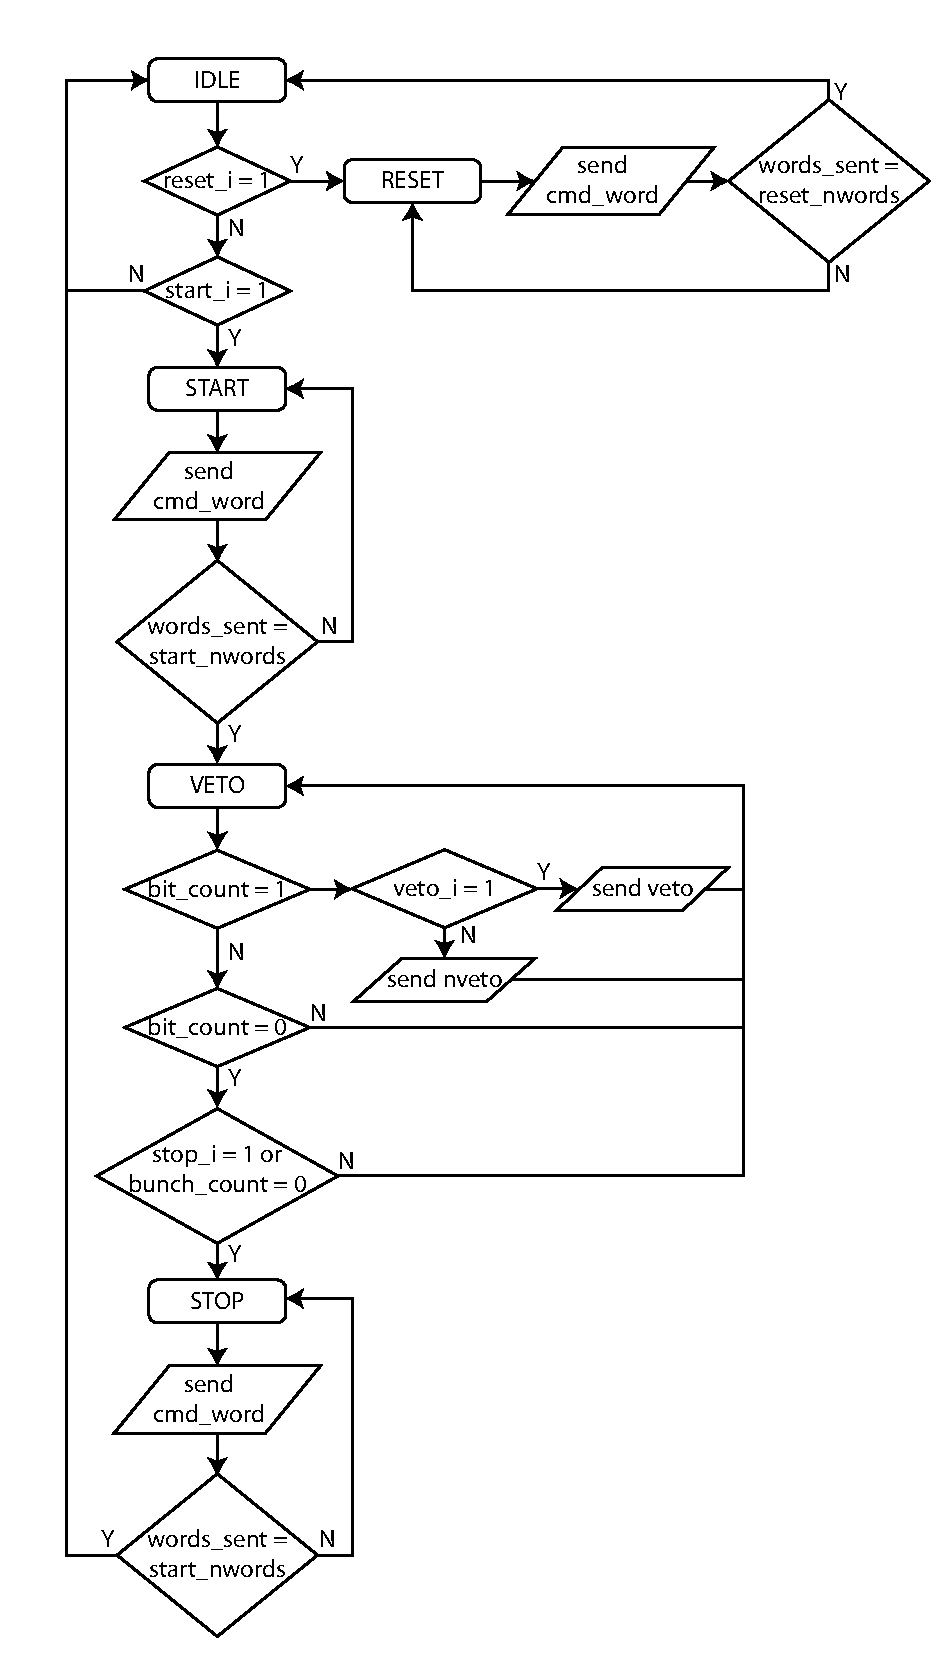
\includegraphics[height=0.8\textheight]{images/pdfs/tx_sm_flow.pdf}
  \caption{Schematic of the control flow in the transmitter entity.}
  \label{fig:tx_sm_flow}
\end{figure}
  
\begin{figure}[htbp]
  \centering
  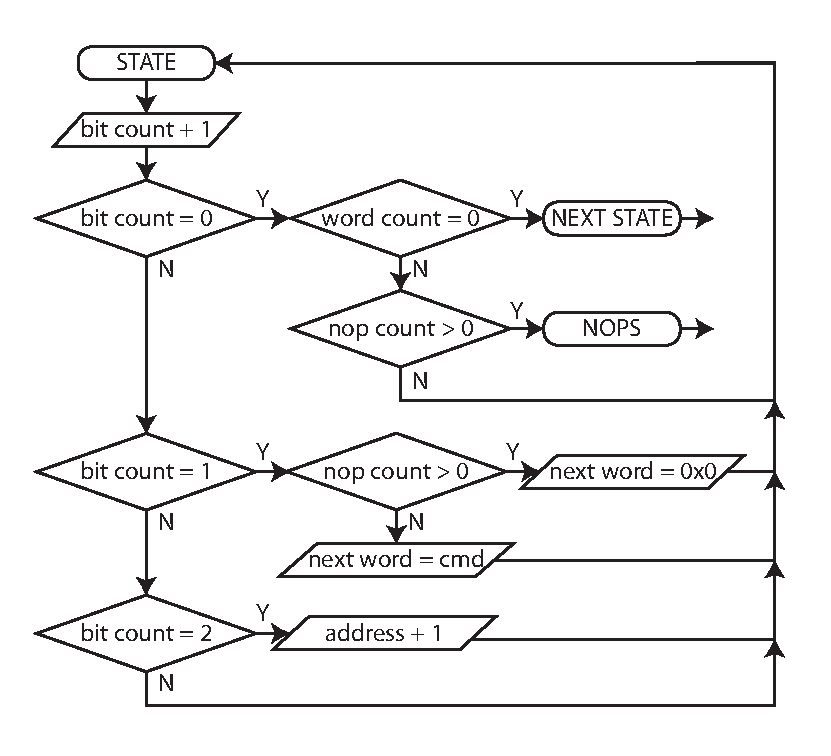
\includegraphics[width=0.7\textwidth]{images/pdfs/tx_sm_bram_control_flow.pdf}
  \caption{General control logic flow for START, STOP and RESET states.}
  \label{fig:tx_sm_bram_control_flow}
\end{figure}
% subsection tx_implementation (end)
% section transmitter (end)
%%%%%%%%%%%%%%%%%%%%%%%%%%%%%%%%%%%%%%%%%%%%%%%%%%%

% chapter implementation (end)
%%%%%%%%%%%%%%%%%%%%%%%%%%%%%%%%%%%%%%%%%%%%%%%%%%%
\chapter{Testing} % (fold)
\label{cha:testing}
This chapter is concerned with the testing regime used on the design. It is split into two sections, first the methodology is discussed and then the results. The aim of testing is to ensure that firstly the design meets the requirements (see chapter~\ref{cha:design}) and secondly that the limitations of the system are understood.
\section{Methodology} % (fold)
\label{sec:methodology}
The methodology used for testing was to iterate rapidly, working from smaller to larger entities and limiting changes to the outer most entity being tested, changes made in sub-entities restarted the processes from that entity to confirm functionality at each level. 

In order to test the designs `test benches' were written. A test bench is a entity that wraps another, the Unit Under Test (UUT), and generates test inputs UUT so its behaviour can be checked. These simulated inputs can be single signals, words or clocks. The UUT and test bench are then simulated and run using a program called, in this case called `iSim', which gives complete control over the system, this means that the response of sub-units can be tested as well as top-level entities. iSim generates an output that is similar to an oscilloscope view with green traces representing boolean values (`1' or `0') and other colours for the other std\_logic values (e.g.\ orange corresponds to `U'). 

% section methodology (end)
\section{Results} % (fold)
\label{sec:results}
While each individual entity was tested, for brevity only the top level tests are included here as they describe the full functionality of the firmware. There are six tests that were run: a simple dynamic run (\texttt{START}\(\rightarrow\)\texttt{NO-VETO}\(\rightarrow\)\texttt{STOP}); veto/no-veto state changes; response to reset command; stop with down-scaler (a requirement for the v~1.0 ASIC); RDMA interface test; and a LocalLink interface test.

For all of these tests there were a couple of pass requirements:
\begin{itemize}
  \item Correct command to response matching.
  \item Synchronicity with the bunch clock
  \item Fixed latency between commands and responses. 
  \item Correct state changes.
\end{itemize}

In the following diagrams the green portions correspond to the iSim traces, the red and blue lines have been added afterwards and indicate chains of causation and serialised command words respectively, the larger yellow dashed lines were also added and indicate bunch trains synchronised to the \texttt{clk\_to\_asic}. On the left hand side are the signal names as used in the design, note that these may not always match the names given in the previous implementation sections.

In all of these tests the clock speed was set to 100~MHz.

\subsection{Start, no-veto, stop} % (fold)
\label{sec:start_no_veto_stop}
Figure~\ref{fig:isim_start-veto-stop} shows a very simple dynamic sequence with a single no-veto word being sent prior to stopping. The top six lines show the \texttt{clk}, \texttt{rst} signals; the transmitter's state (\texttt{current\_state}); the simulated input from the CCC (\texttt{cmd} and \texttt{veto}); and the output to the ASIC (\texttt{cmd\_to\_asic}).

After the \texttt{START} signal is received from the CCC the appropriate flag (\texttt{start\_from\_rx}) is set, followed by the delayed flag (\texttt{start\_delayed}) to the transmitter, which starts sending the appropriate command set.\footnote{The first word to the ASIC is \texttt{RSYNC} so begins with a `0' rather than `1'.} The delayed flag then forms the \texttt{log\_start} and \texttt{veto\_start} signals that indicate when to log the header information and start logging vetoes respectively. Meanwhile the \texttt{NO-VETO} signal is received and combined with the \texttt{veto\_start} to form flag that the transmitter should send a \texttt{TRIGGER\_FLAG\_SET}. Finally the \texttt{STOP} signal is received, triggering the stop sequence and ultimately a return to IDLE (not shown).

Based on the general requirements it's clear that the correct responses are being sent (and hence the state-changes are occurring as required), the commands are synchronised with the bunch clock and the latency is as required: 6~clocks for commands and 7 for vetoes (the extra length for vetoes is due to the three rather than four bit command).

\begin{sidewaysfigure}[H]
    \centering
    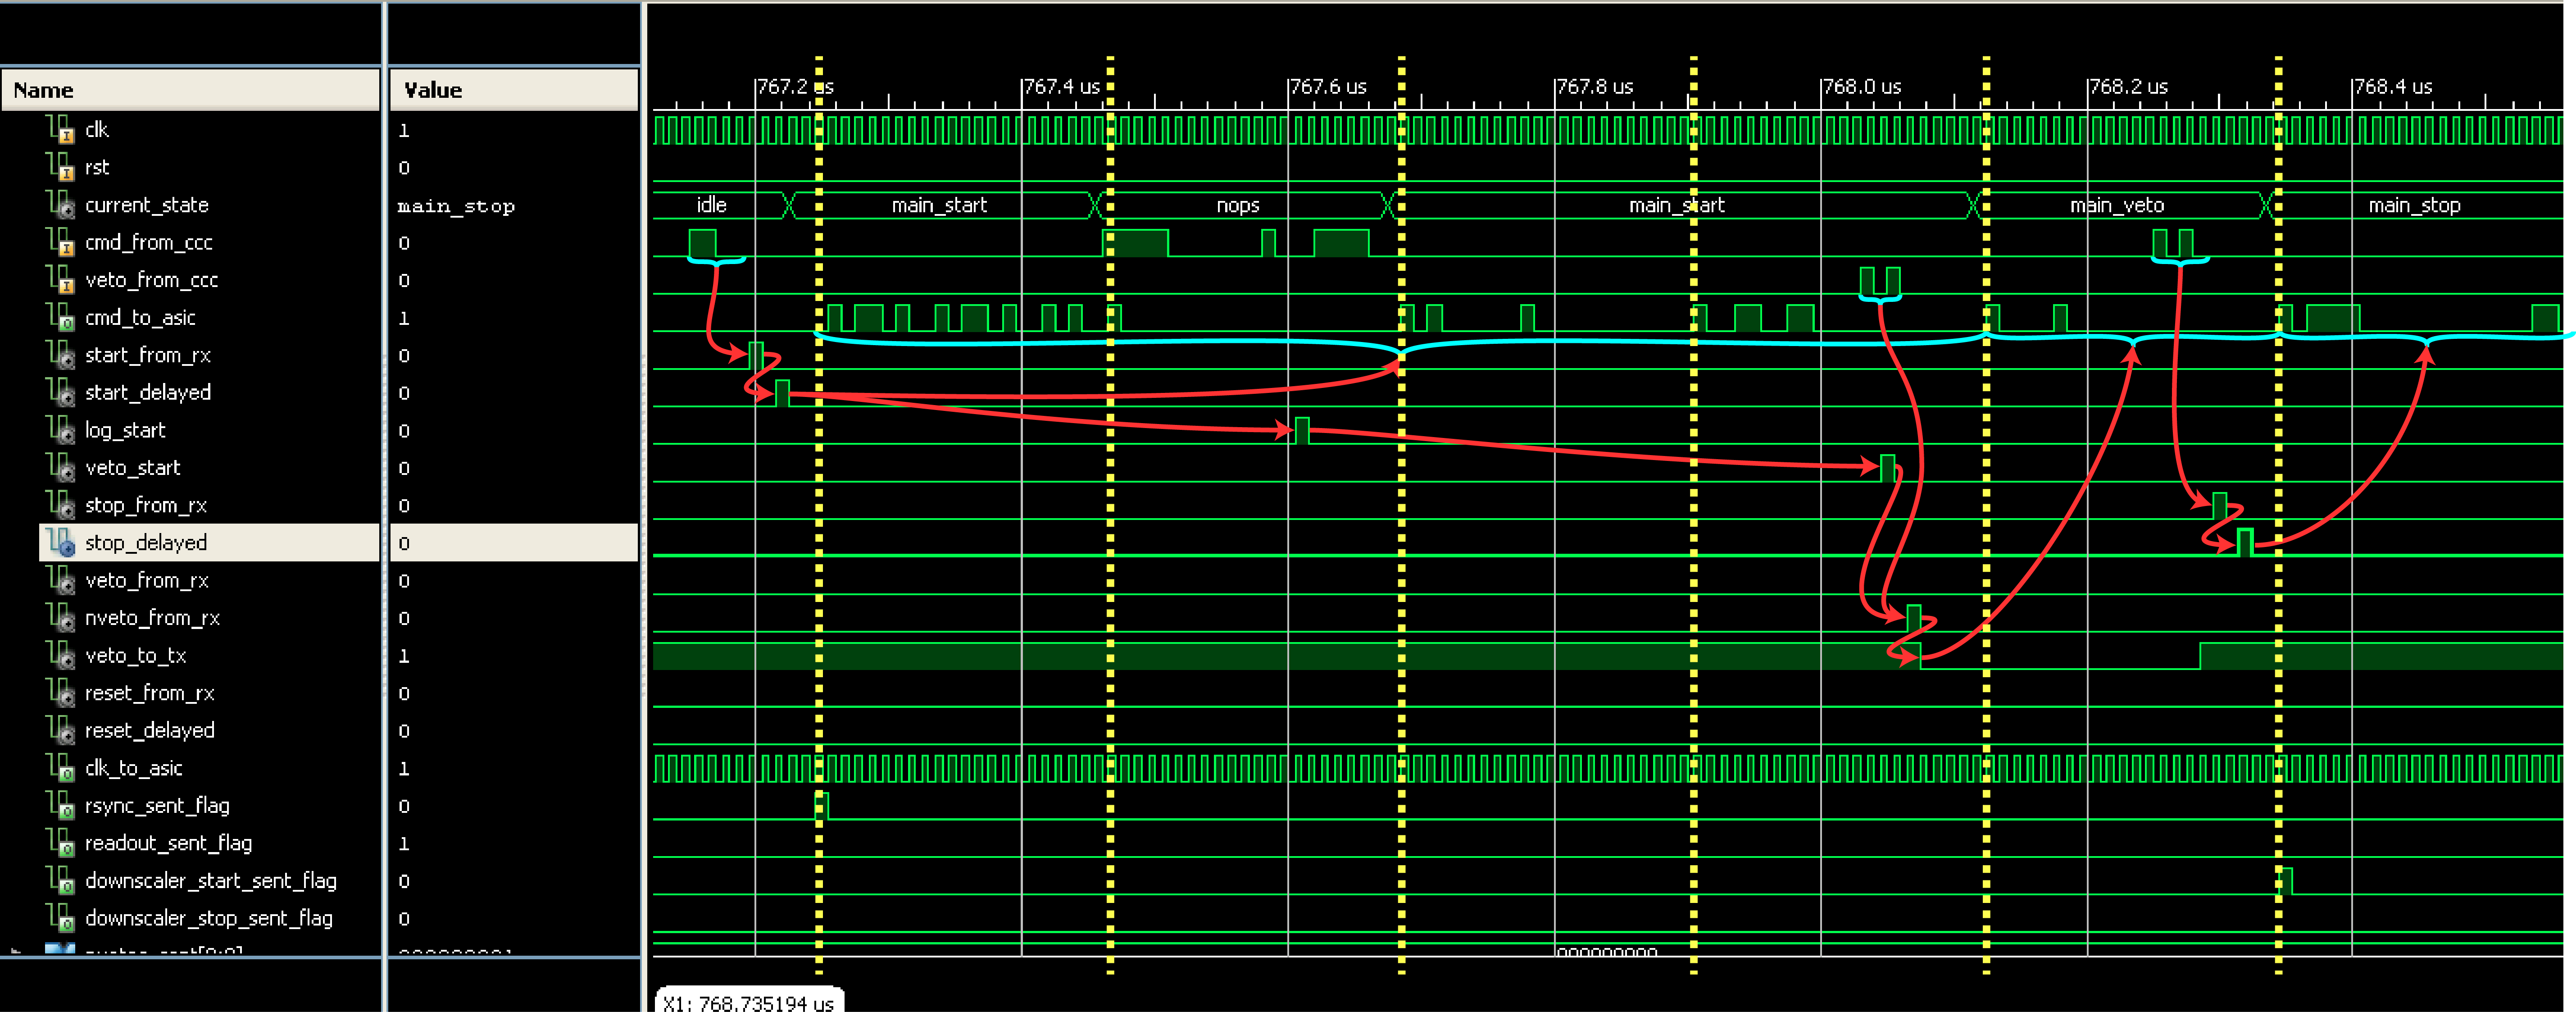
\includegraphics[width=\textwidth]{images/isim/edited/start-veto-stop.png}
    \caption{A \texttt{START}, \texttt{NO-VETO}, \texttt{STOP} sequence with a single \texttt{NO-VETO} prior to the stop signal. The blue braces indicate either input/output word sequences whilst the red lines show logical sequences.}
    \label{fig:isim_start-veto-stop}
\end{sidewaysfigure}

% subsection start_no_veto_stop (end)
\clearpage
\subsection{Veto/No-veto} % (fold)
\label{sec:veto_no_veto}
Figure~\ref{fig:isim_veto_no_veto} shows the dynamic veto mode in operation, 3 vetoes followed by 6 no-vetoes. The main lines to note are between \texttt{veto\_from\_ccc} and \texttt{veto\_to\_tx}. The general operation is: first the signal is received and flagged (on either of the two lines, \texttt{veto\_from\_rx} and \texttt{nveto\_from\_rx}), the decision is made by the veto-filter (\texttt{veto\_to\_tx}) and the response sent to the ASIC. The different responses can be seen in the single \texttt{NOP} for \texttt{VETO}s whilst the \texttt{TRIGGER\_FLAG\_SET} (0x10) is sent for \texttt{NO-VETO}. 

\begin{sidewaysfigure}[H]
  \centering
  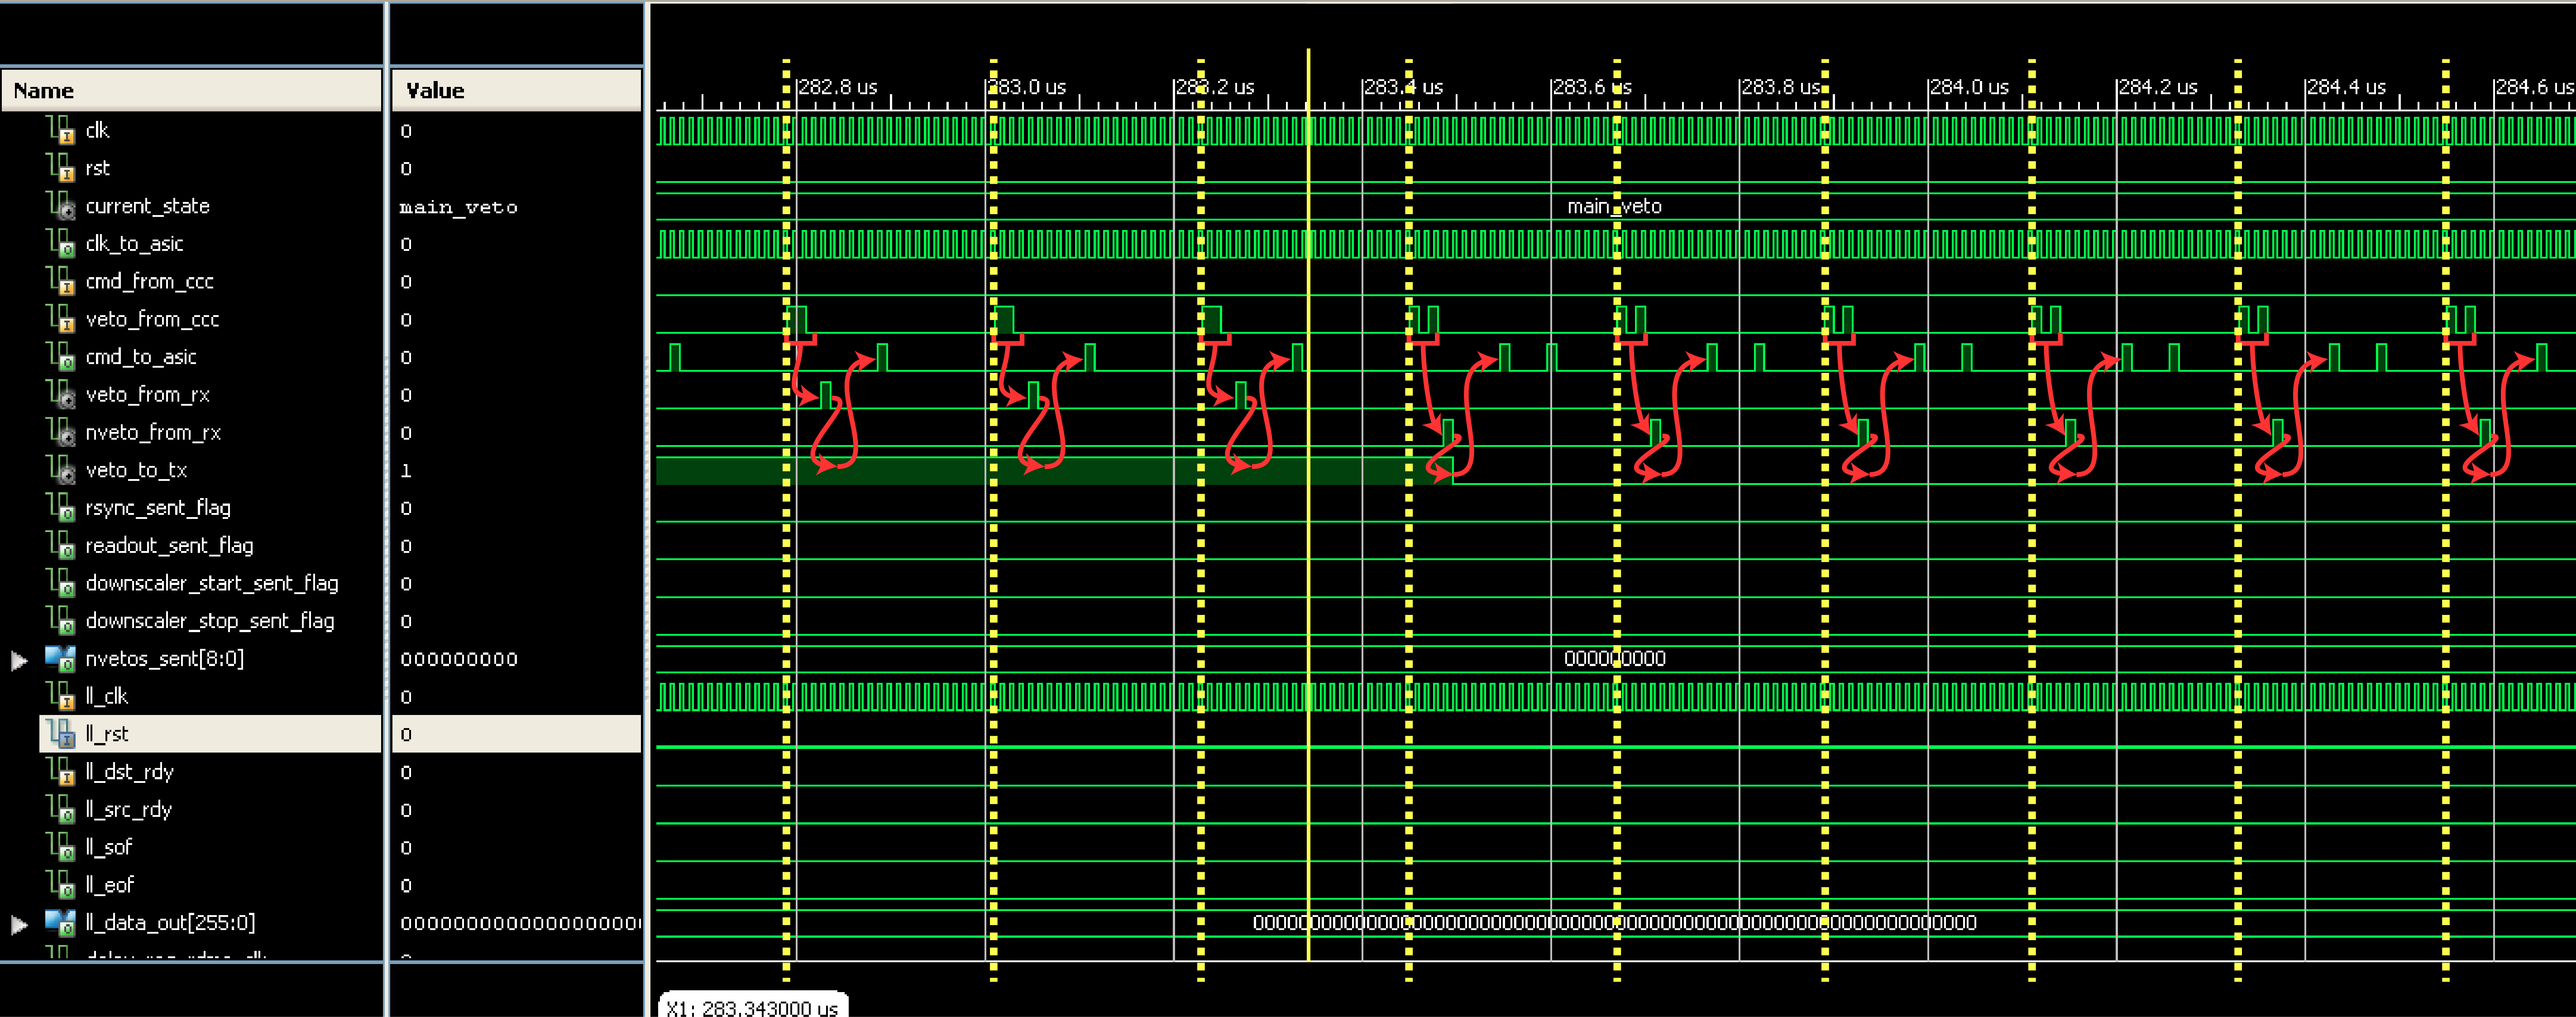
\includegraphics[width=\textwidth]{images/isim/edited/veto_no_veto.png}
  \caption{A selection of vetos/no-vetos.}
  \label{fig:isim_veto_no_veto}
\end{sidewaysfigure}
% subsection veto_no_veto (end)
\clearpage
\subsection{Reset Command} % (fold)
\label{sec:reset_command}
Figure~\ref{fig:isim_reset_cmd} shows the reset sequence being sent in response to the \texttt{RESET} command from the CCC, first the word arrives, then we see the delayed signal from the receiver and then the thee words sent to the ASIC. The first word of the \texttt{RESET} command sequence is a \texttt{RSYNC} so the \texttt{rsync\_sent\_flag} is asserted also it contains a \texttt{NOP} command so the appropriate state change occurs and a single \texttt{NOP} is sent. Figure~\ref{fig:isim_reset_rdma} shows the same process being triggered via the control register which is set via RDMA, i.e.\ the `reset-mode'.
\begin{sidewaysfigure}[H]
  \centering
  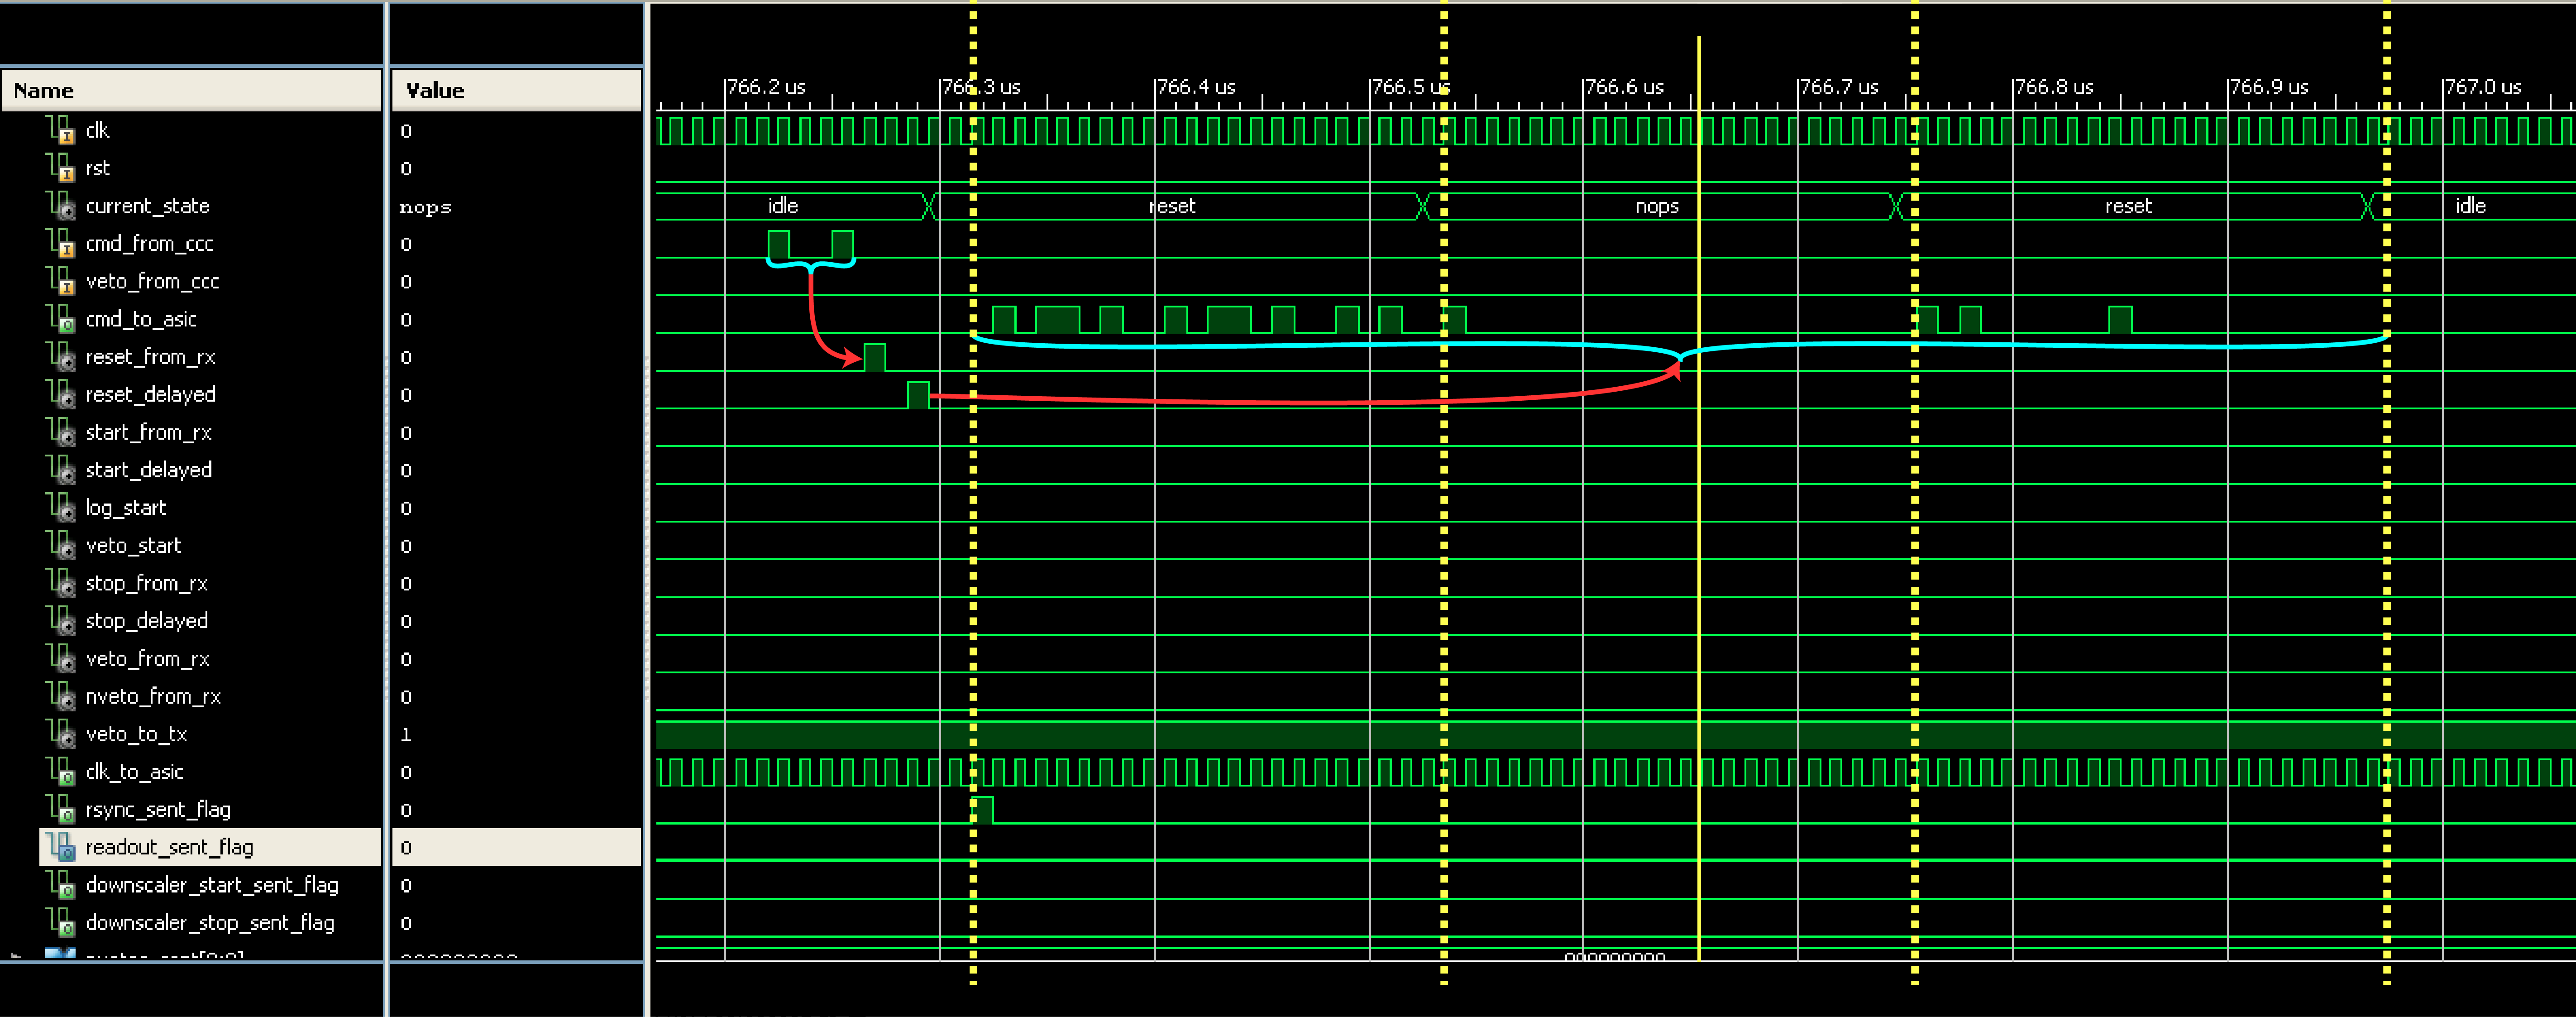
\includegraphics[width=\textwidth]{images/isim/edited/reset_cmd.png}
  \caption{The reset sequence being triggered by the cmd line from the CCC.}
  \label{fig:isim_reset_cmd}
\end{sidewaysfigure}
\begin{sidewaysfigure}[H]
  \centering
  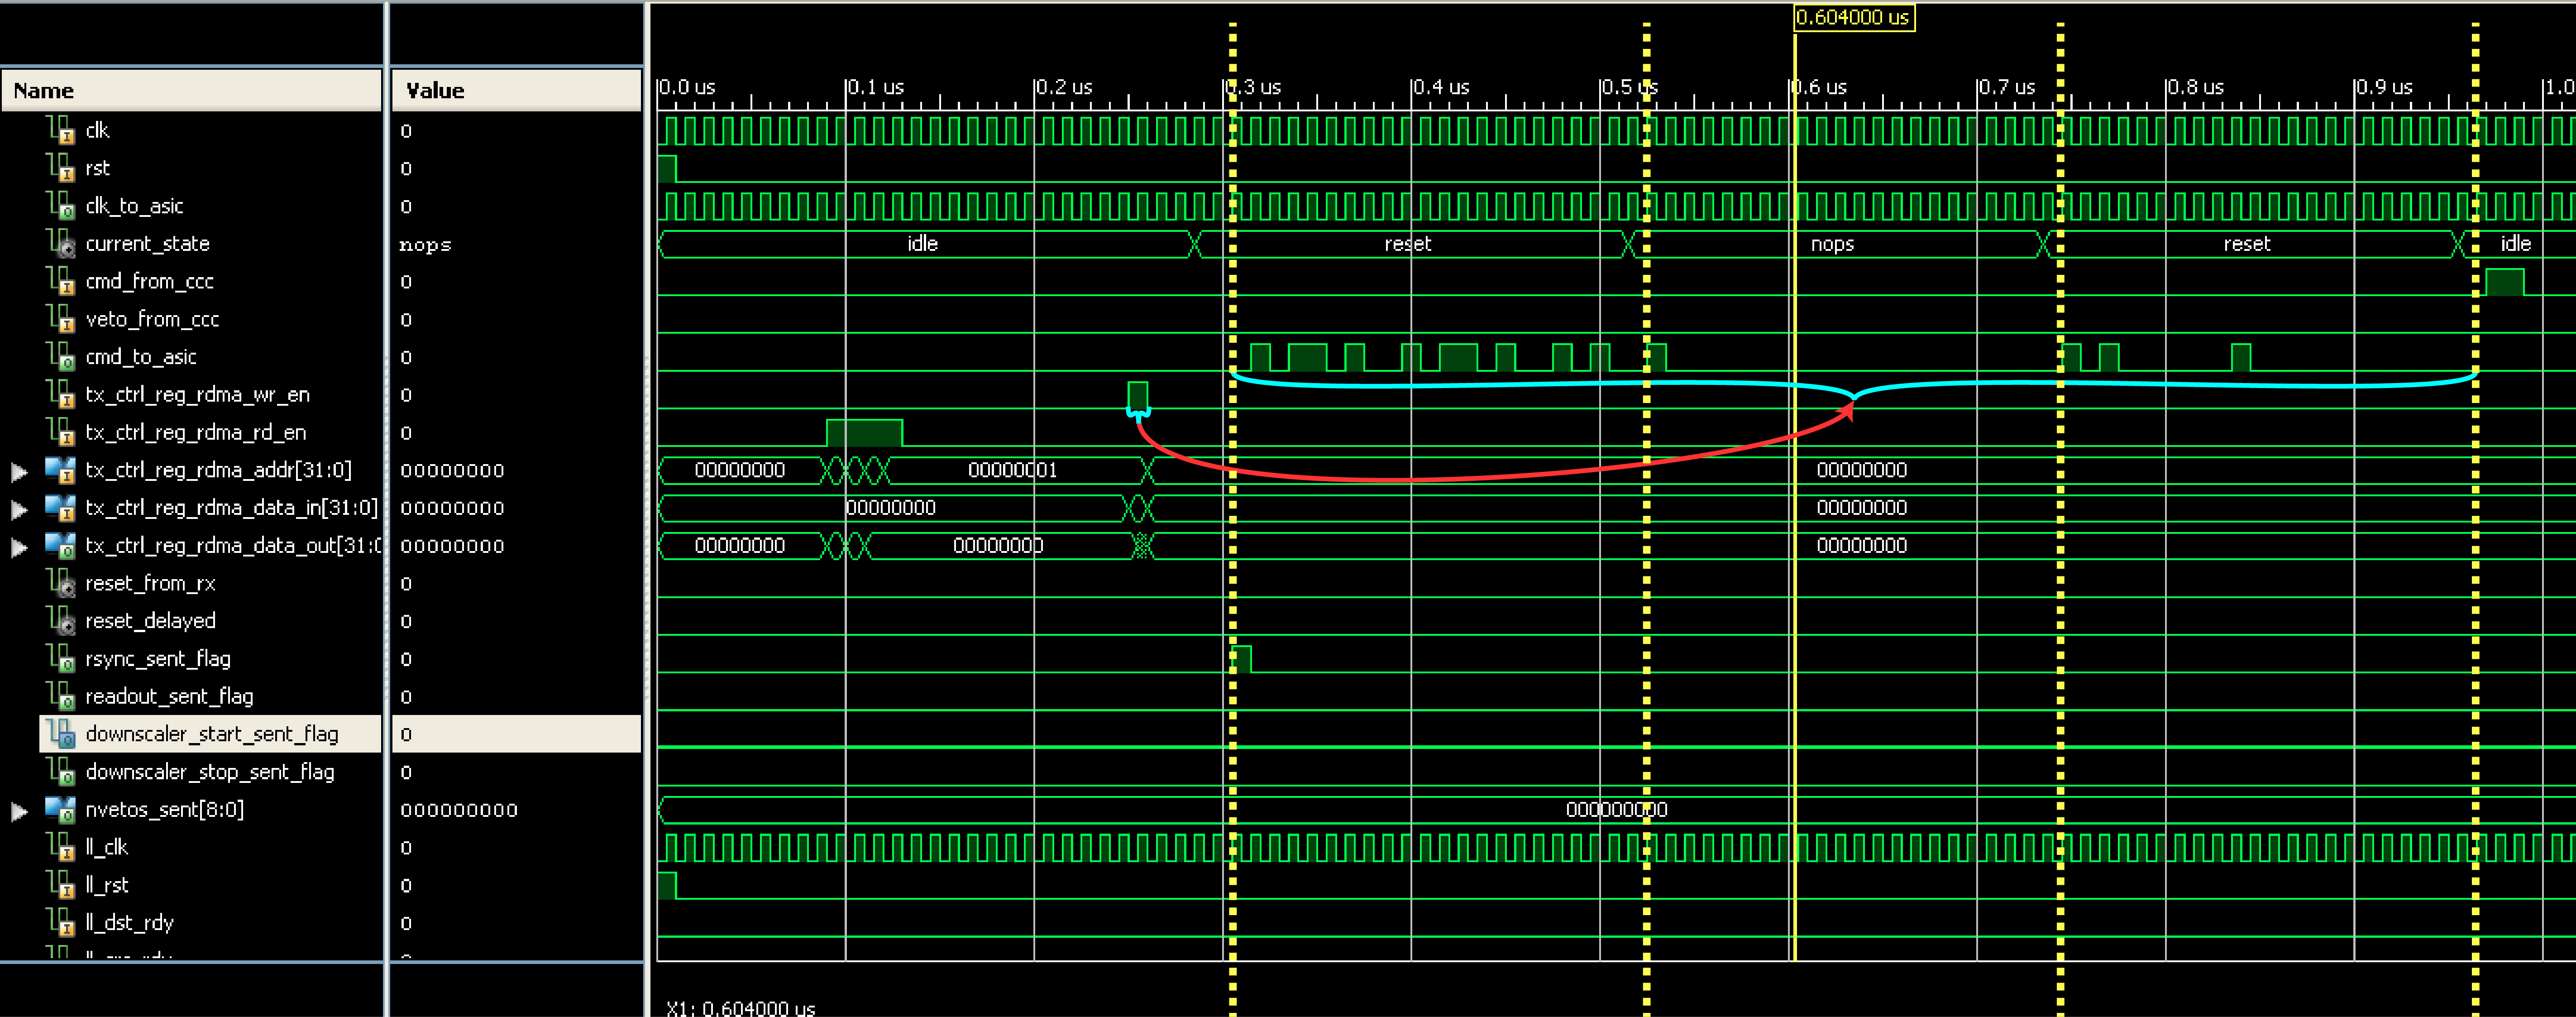
\includegraphics[width=\textwidth]{images/isim/edited/reset_rdma.png}
  \caption{The reset sequence being triggered via the control register.}
  \label{fig:isim_reset_rdma}
\end{sidewaysfigure}
% subsection reset_command (end)
\clearpage
\subsection{Stop with down-scaler} % (fold)
\label{sec:stop_downscaler}
For this test the operation of the down-scaler for the v~1.0 ASIC checked. Prior to the yellow-dashed line in figure~\ref{fig:isim_stop-downscaler} the \texttt{clk\_to\_asic} is running at 100~MHz, after it runs at 1~MHz. The order of events is more clearly show in the close up, figure~\ref{fig:isim_stop-downscaler-zoom}, which corresponds to the region between the dashed and solid lines in figure~\ref{fig:isim_stop-downscaler}. Once the \texttt{STOP} command is received the first word, the down-scaler trigger, is sent to the ASIC, once this is sent the next word (in this case \texttt{READ\_OUT\_DATA}) is sent at the selected speed. Note that the \texttt{READ\_OUT\_DATA} flag is set and held for one clock at the down-scaled speed.

\begin{sidewaysfigure}[H]
  \centering
  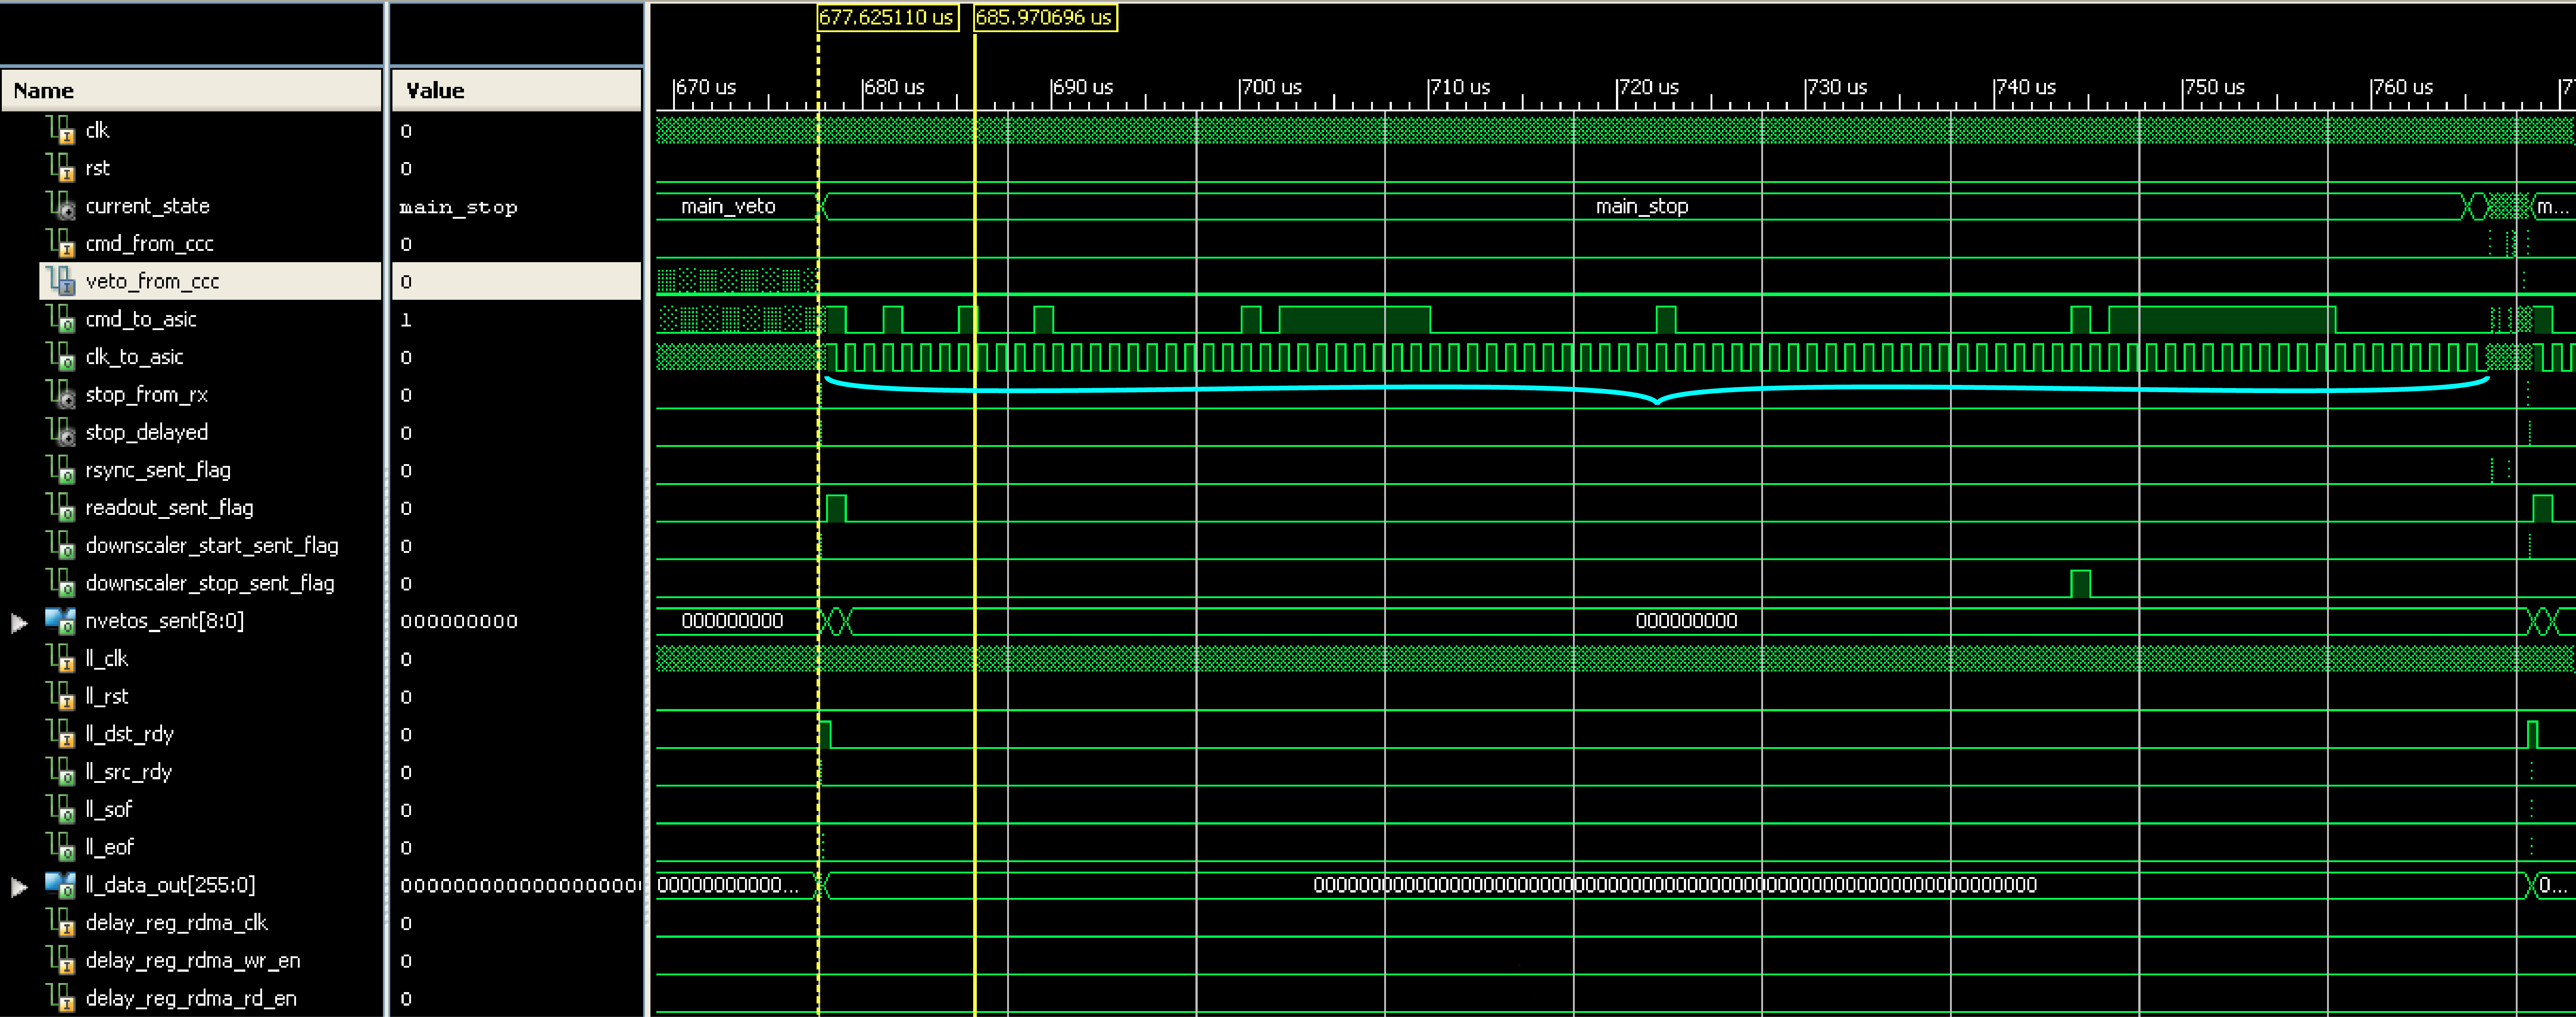
\includegraphics[width=\textwidth]{images/isim/edited/stop-downscaler.png}
  \caption{The \texttt{clk\_to\_asic} down-scaled by a factor of 100. The section delimitated by the yellow guides is shown in figure~\ref{fig:isim_stop-downscaler-zoom}. Note that the second word sent (after the down-scaler trigger) is the \texttt{READ\_OUT\_START} command, the flag is also down-scaled.}
  \label{fig:isim_stop-downscaler}
\end{sidewaysfigure}
    
\begin{sidewaysfigure}[H]
  \centering  
  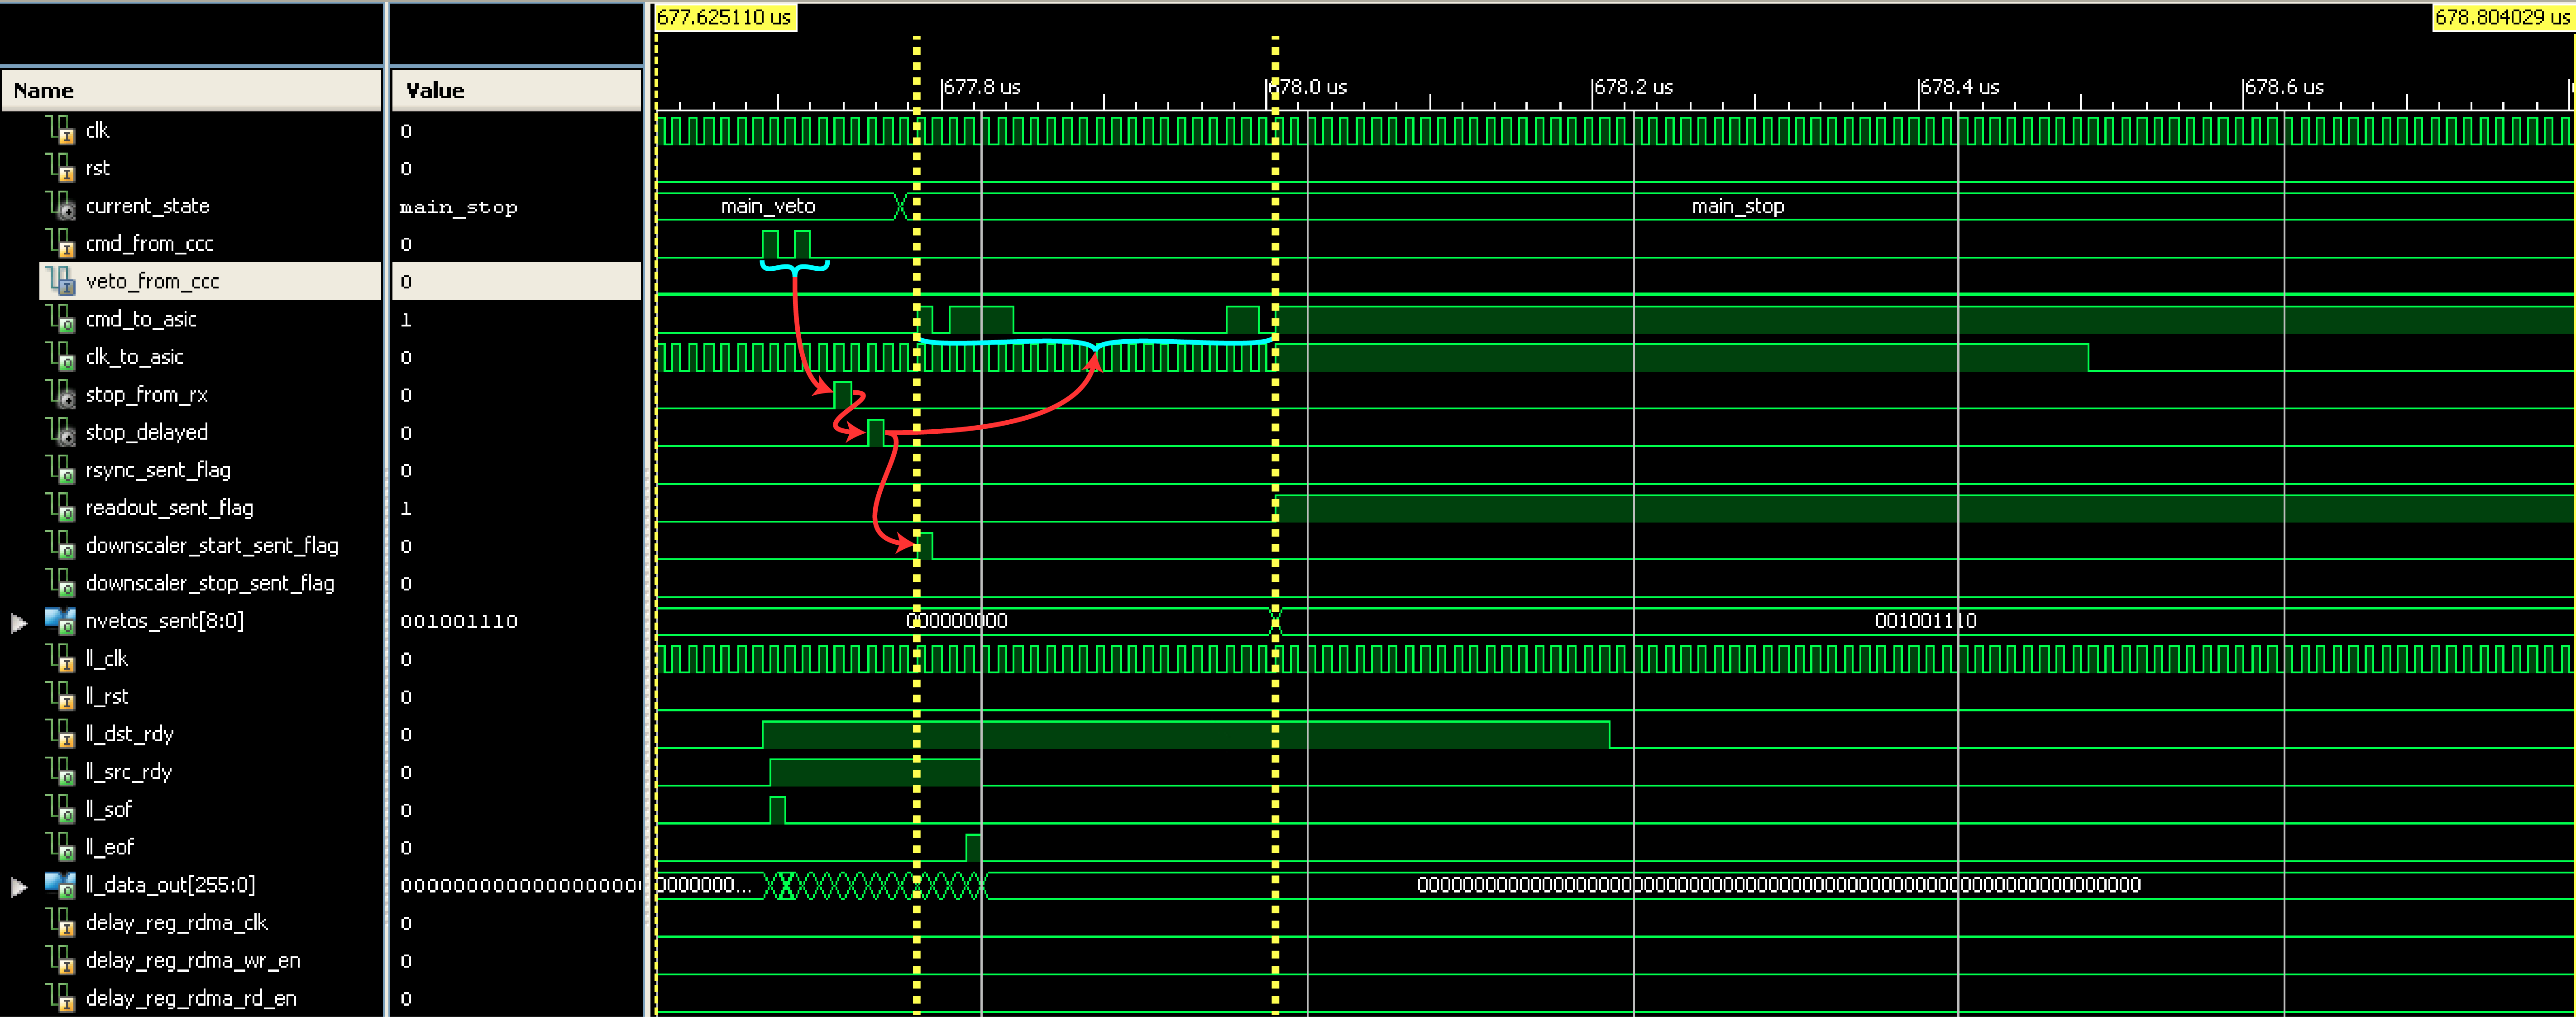
\includegraphics[width=\textwidth]{images/isim/edited/stop-downscaler-zoom.png}
  \caption{The \texttt{STOP} command and down-scaler start word being sent. Note the LocalLink transfer on the `ll\_' lines.}
  \label{fig:isim_stop-downscaler-zoom}
\end{sidewaysfigure}
% subsection stop_downscaler (end)
\clearpage
\subsection{RDMA} % (fold)
\label{sec:rdma}
Figure~\ref{fig:isim_rdma} shows a simple test of the RDMA accessible registers and BRAMs. The first four addresses of each entity is read out. These were checked by hand against the values written at the start.
\begin{sidewaysfigure}[H]
  \centering
  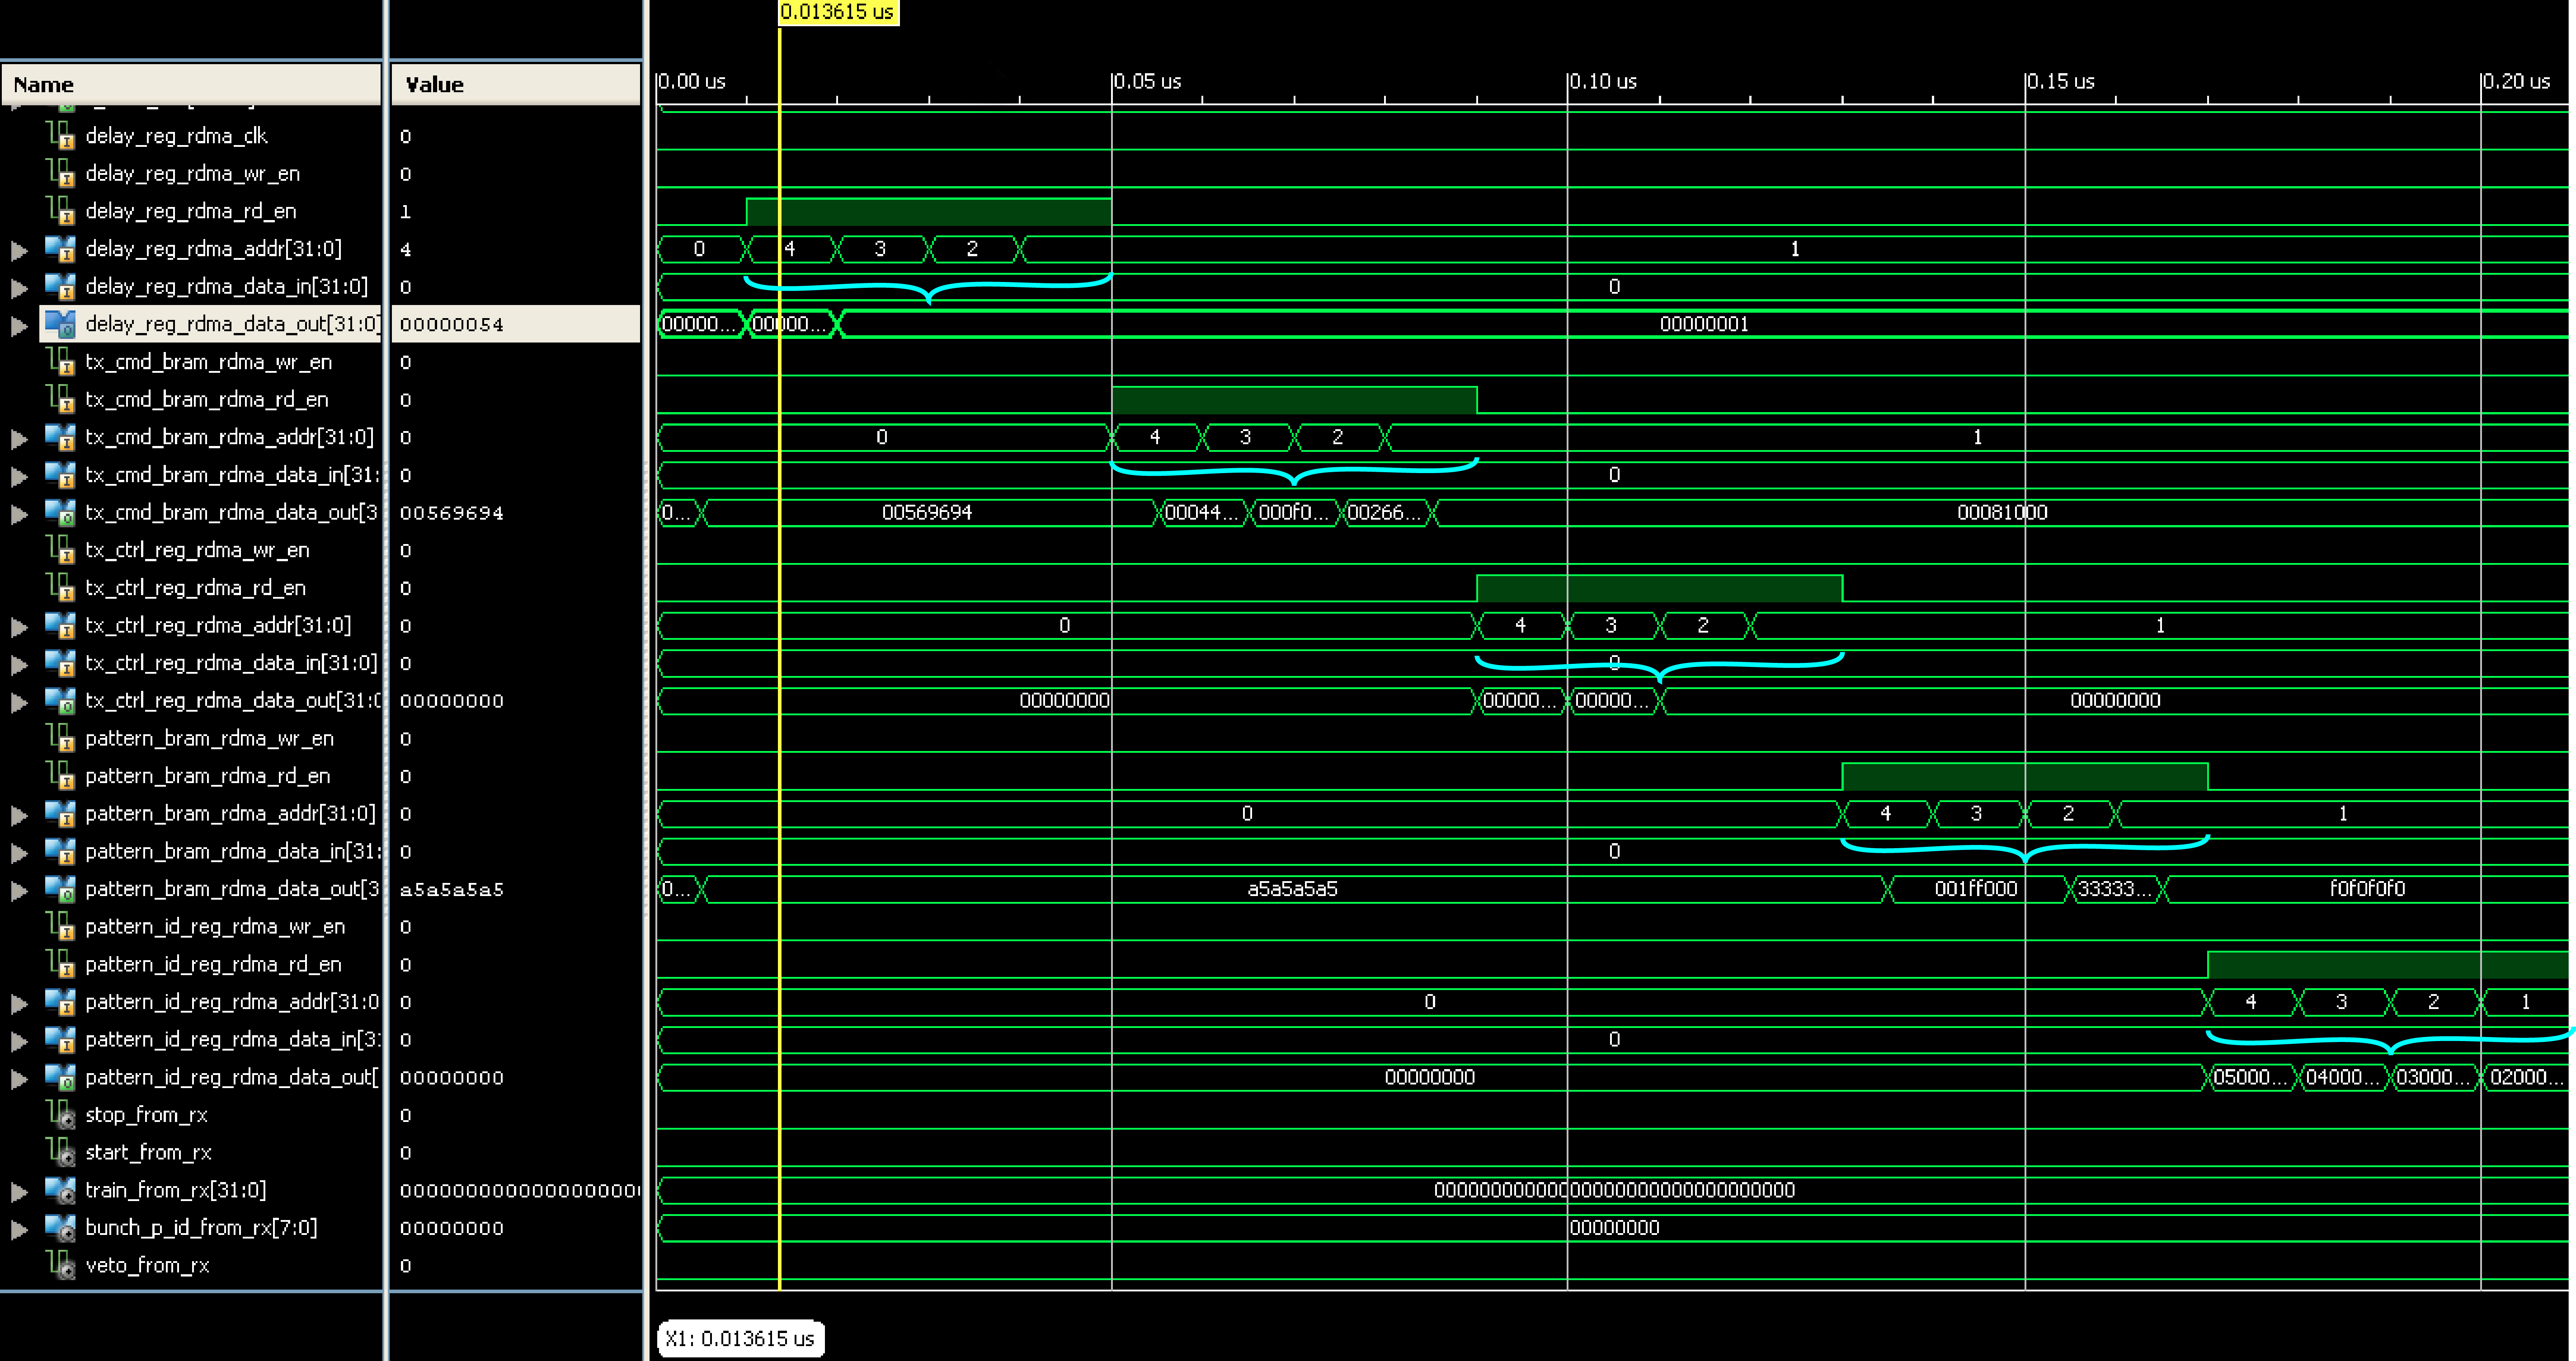
\includegraphics[width=\textwidth]{images/isim/edited/rdma.png}
  \caption{Read back of the first 4 locations of every entity accessible via RDMA.}
  \label{fig:isim_rdma}
\end{sidewaysfigure}
    
% subsection rdma (end)
\clearpage
\subsection{Local Link} % (fold)
\label{sec:local_link}
A sample read-out of the veto-log is shown in figure~\ref{fig:isim_locallink}. The LocalLink specification requires that data transfer starts as soon as both source and destination are read. In this test all bunches were vetoed apart from the first \(n\) of each 256 bunches (where \( n\) is the \( n^{th} \) block of 256 bunches), this resulted in the top bits being filled with 0's; the first word is 0-padded and contains the header information (i.e.\ the train ID and the bunch pattern ID).
\begin{sidewaysfigure}[H]
  \centering
  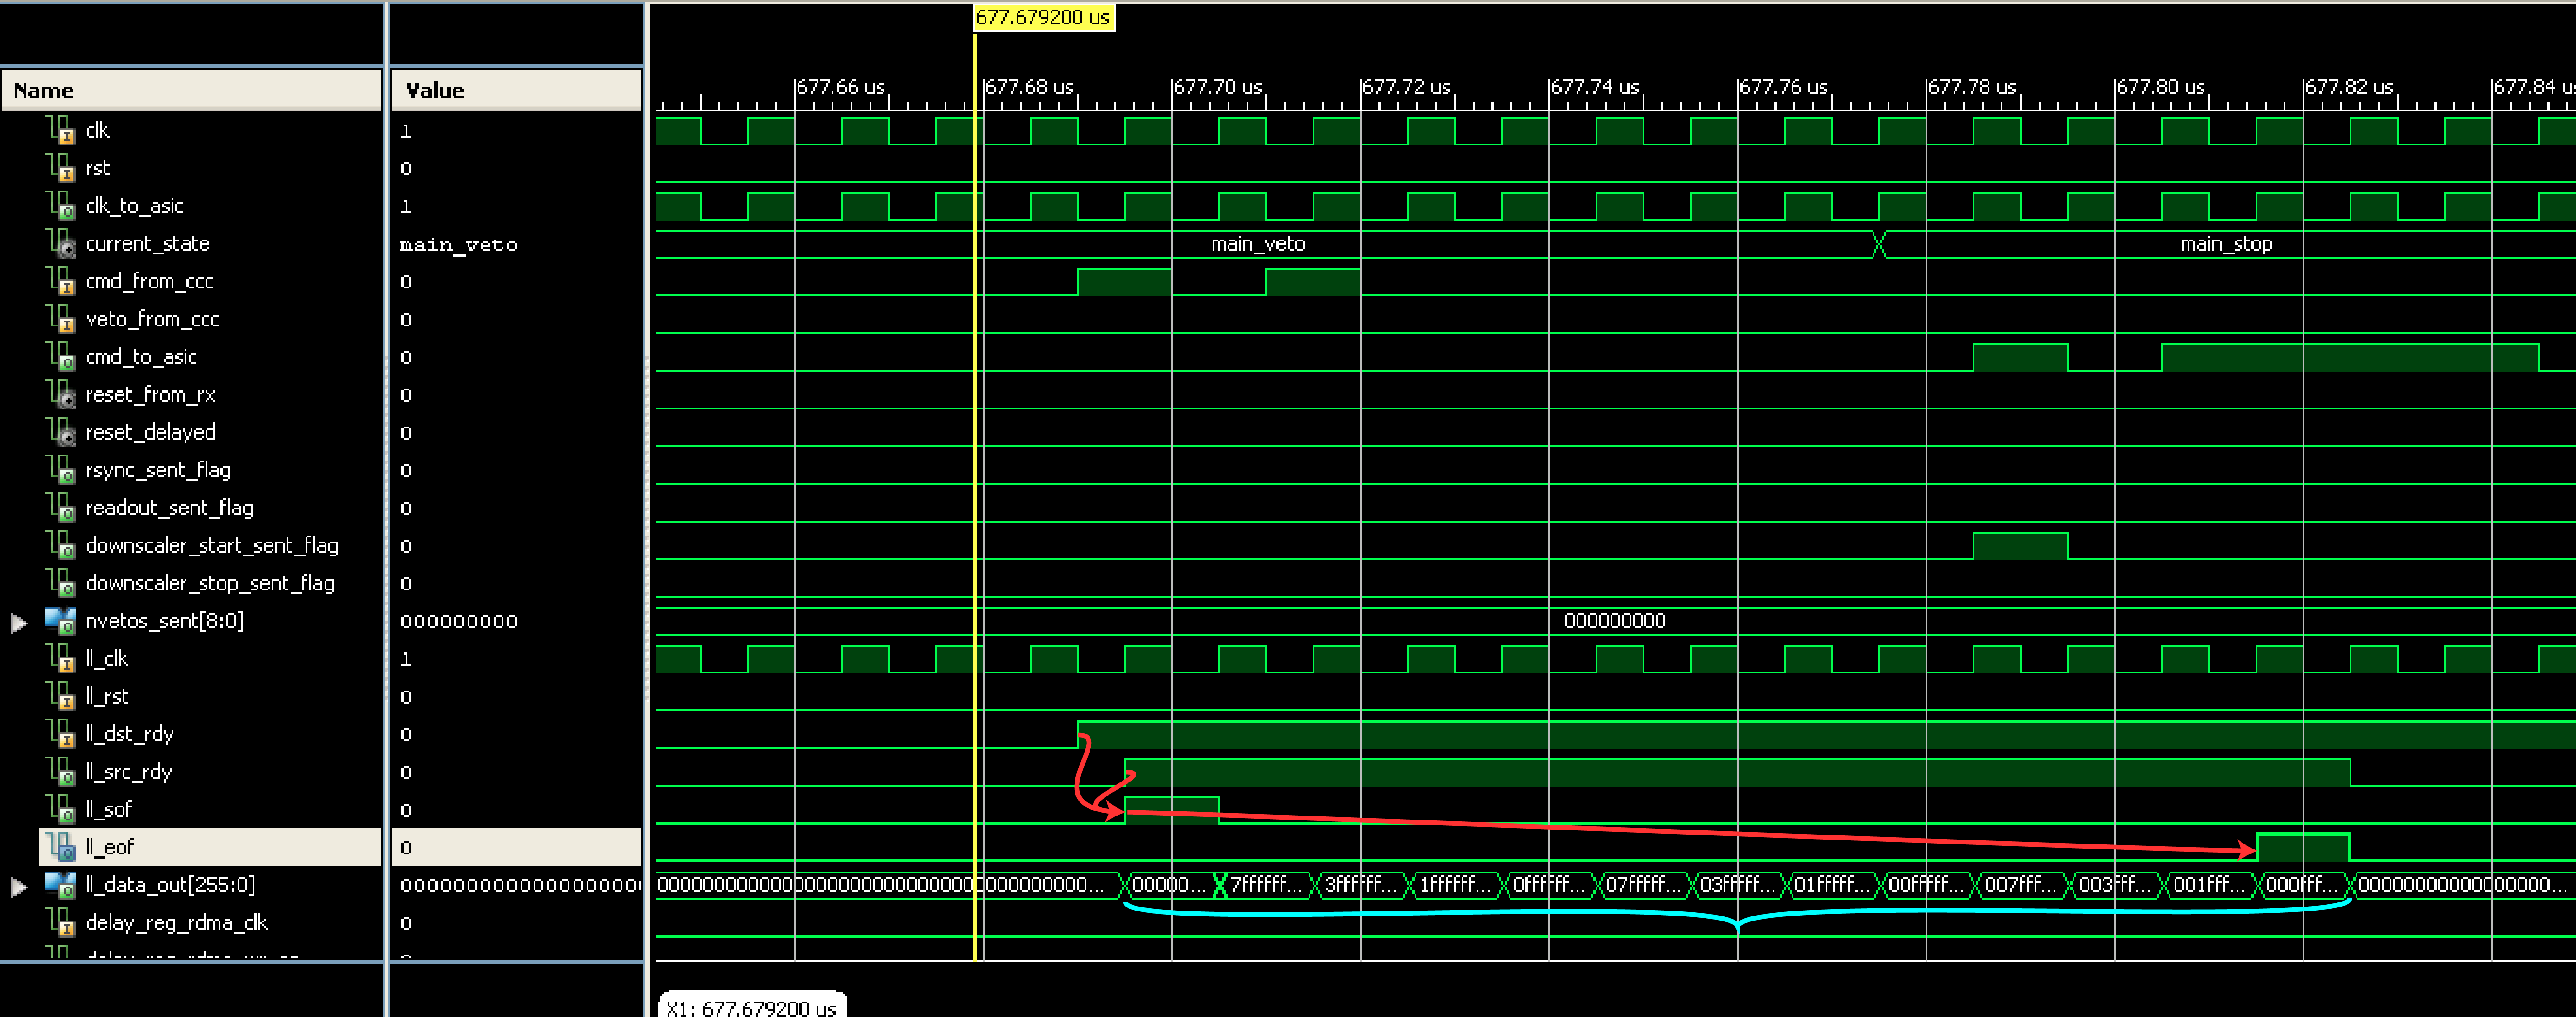
\includegraphics[width=\textwidth]{images/isim/edited/locallink.png}
  \caption{Read-out of the veto log for 3072 bunches.}
  \label{fig:isim_locallink}
\end{sidewaysfigure}
    
% subsection local_link (end)
\clearpage
% section results (end)
%%%%%%%%%%%%%%%%%%%%%%%%%%%%%%%%%%%%%%%%%%%%%%%%%%%
% chapter timing_diagrams (end)
%%%%%%%%%%%%%%%%%%%%%%%%%%%%%%%%%%%%%%%%%%%%%%%%%%%
\chapter{Conclusion} % (fold)
\label{cha:conclusion}
EuXFEL is a huge project, 3.4~km of systems and sub-systems that must be kept in sync at all times in order to work. One of these many sub-systems is the LPD, one of three planned 2D pixel detectors, that will record up to 5,120\( \times \)1~Mpixel images every second. Control of this detector is achieved via 16 FEMs each of which uses a command signal and clock signal, distributed to its supermodule of 512 ASICs, to maintain order. To provide a simple interface between the 2D detectors and the rest of EuXFEL the CCC uses three lines to distribute a \( \sim \)99~MHz clock, a fast command signal, and a veto signal whilst receiving status information. 

The LPD-CCC interface firmware runs on the FEM and provides translation from the three received signals to the two that each ASIC expects. This interface was split into three entities that dealt with receiving, vetoing and transmitting the information from the CCC. Using a rigorous testing regime each entity was developed according to the requirements of both LPD and CCC. The final designs use a combination of state-machines and BRAM to respond rapidly and accurately to each in-bound signal.

Whilst EuXFEL is several years off of operation the interface is already proving its mettle having been used in a recent beam test of the LPD detector at LCLS and in test benches for the CCC board itself.

% chapter conclusion (end)
%%%%%%%%%%%%%%%%%%%%%%%%%%%%%%%%%%%%%%%%%%%%%%%%%%%
\appendix
\chapter{EuXFEL Appendix} % (fold)
\label{cha:appendix}
\section{ASIC command words} % (fold)
\label{app:asic_command_words}
The table~\ref{tab:asic_command_words} provides a full list of all commands implemented by the LPD ASIC, for discussion of what they do see the LPD manual~\cite{lpd_manual}.

\begin{table} [htbp]
  \begin{center} 
    \setlength{\extrarowheight}{1.5pt}
    \begin{tabular}{c | l || c|l}
      Word & Name &  Word & Name \\
      \hline  
      0x00 & NOP                      &  0x0D    & RESET\_TRIGGER\_POINTER     \\
      0x01 & STAND\_BY                &  0x0E    & START\_WRITE\_POINTER       \\
      0x02 & POWER\_UP                &  0x0F    & START\_TRIGGER\_POINTER     \\
      0x03 & ON\_CHIP\_RESET\_DISABLE &  0x10    & TRIGGER\_FLAG\_SET          \\
      0x04 & ON\_CHIP\_RESET\_ENABLE  &  0x11    & READ\_OUT\_DATA             \\
      0x05 & RESET\_PRE\_AMP          &  0x12    & REMOVE\_RESET\_PRE\_AMP     \\
      0x06 & RESET\_GAIN\_FRONT       &  0x13    & REMOVE\_RESET\_GAIN\_STAGE1 \\
      0x07 & RESET\_GAIN\_BACK        &  0x14    & REMOVE\_RESET\_GAIN\_STAGE2 \\
      0x08 & Reserved                 &  0x15    & CLOCK\_DIV\_SEL             \\
      0x09 & TEST\_MODE\_D            &  0x16    & SELF\_TEST\_EN              \\
      0x0A & TUNE\_MODE               &  0x17    & STOP\_READ\_OUT             \\
      0x0B & CLEAR\_SKIP\_REGISTER    &  0x18    & RESET\_STATE\_MACHINE       \\
      0x0C & RESET\_WRITE\_POINTER    &  0x5A5A5 & SYNC\_RESET                 \\
    \end{tabular}
  \end{center}
  \caption{ASIC command words, see \cite{lpd_manual} for a full description and recommended use of these commands.}
  \label{tab:asic_command_words}
\end{table}
% section asic_command_words (end)
%%%%%%%%%%%%%%%%%%%%%%%%%%%%%%%%%%%%%%%%%%%%%%%%%%%
\section{RDMA interface} % (fold)
\label{app:rdma_interface}
The RDMA interfaces used throughout the project have the interface seen in table~\ref{tab:rdma_interface}. The appropriate mask for the address is given in appropriate interface notes. In general for BRAMs a size of 32\(\times\)1024 the appropriate bits are 9:0 whilst for registers the bits 3:0 are used. 
    
\begin{table}[htbp]
  \begin{center}
    \begin{tabulary}{\textwidth}{l|c|c|L}
      Name & Direction & Type & Notes \\
      \hline
      clk       & \multirow{6}{*}{in}
      & sl                & The RDMA clock (this can be separate from e.g. the CCC clock).\\
      rst       &     & sl                & Reset the memory to some default state.                       \\
      rd\_en    &     & sl                & Enable read operations at the address.                        \\
      wr\_en    &     & sl                & Enable write operations at the address.                       \\
      addr      &     & slv (31:0) & The address the MSB will be masked.                           \\
      data\_in  &     & slv (31:0) & Used for writing and otherwise ignored.                       \\
      \hline
      data\_out & out & slv (31:0) & Data out, only guaranteed for read operations.                \\
        
    \end{tabulary}
  \end{center}
  \caption{Standard RDMA interface.}
  \label{tab:rdma_interface}
\end{table}
% section rdma_interface (end)
%%%%%%%%%%%%%%%%%%%%%%%%%%%%%%%%%%%%%%%%%%%%%%%%%%%
\section{Local Link interface} % (fold)
\label{app:local_link_interface}
The Local Link~\cite{locallink_spec} interface is used only to read out the veto log. The details of the frame composition are given in section~\ref{sec:veto_filter}. The interface used is minimal (i.e. no optional features are used) and given in table~\ref{tab:local_link_interface}.
\begin{table}[htbp]
  \begin{center}
    \begin{tabulary}{\textwidth}{l | c | c | L}
      Name & Direction & Type & Notes \\
      \hline
      clk        & \multirow{3}{*}{in} 
      & sl                 & The LL clock (this can be separate from e.g. the CCC clock).\\
      rst        &     & sl                 & Abort.                                                      \\
      dst\_rdy   &     & sl                 & Destination ready.                                          \\
      \hline
      src\_rdy   & \multirow{4}{*}{out}
      & sl                 & Source ready i.e. this entity.                               \\
      sof        &     & sl                 & Start of frame flag.                                        \\
      eof        &     & sl                 & End of frame flag.                                          \\
      data\_out  &     & slv (255:0) & Data out.                                                   \\
    \end{tabulary}
  \end{center}
  \caption{Minimal local link interface as used by the veto logger.}
  \label{tab:local_link_interface}
\end{table}
  
% section local_link_interface (end)
%%%%%%%%%%%%%%%%%%%%%%%%%%%%%%%%%%%%%%%%%%%%%%%%%%%
  
% chapter appendix (end)
